%% The first command in your LaTeX source must be the \documentclass command.
%%
%% Options:
%% twocolumn : Two column layout.
%% hf: enable header and footer.
\documentclass[
% twocolumn,
% hf,
]{ceurart}
\usepackage{physics}
\usepackage[english]{babel}
\usepackage{amsthm}
\usepackage{geometry}
\usepackage{hyperref}
\usepackage{caption}
\usepackage{amsmath}
\usepackage[linesnumbered,ruled]{algorithm2e}
\usepackage{booktabs}
\usepackage{graphicx}
\usepackage{listings}
\usepackage{subcaption}
\usepackage{adjustbox}
\usepackage{siunitx}



\theoremstyle{definition}
\newtheorem{definition}{Definition}[section]

\renewcommand*\descriptionlabel[1]{\hspace\leftmargin$#1$}

%%
%% One can fix some overfulls
\sloppy

\tolerance=1
\emergencystretch=\maxdimen
\hyphenpenalty=10000
\hbadness=10000

%%
%% Minted listings support 
%% Need pygment <http://pygments.org/> <http://pypi.python.org/pypi/Pygments>
\usepackage{listings}
%% auto break lines
\lstset{basicstyle=\fontfamily{pcr}\selectfont\footnotesize}

%%
%% end of the preamble, start of the body of the document source.
\begin{document}

\SetArgSty{textup}



%%
%% Rights management information.
%% CC-BY is default license.
\copyrightyear{2025}
\copyrightclause{Copyright for this paper by its authors.
  Use permitted under Creative Commons License Attribution 4.0
  International (CC BY 4.0).}

%%
%% This command is for the conference information
%\conference{Woodstock'22: Symposium on the irreproducible science,
%  June 07--11, 2022, Woodstock, NY}

%%
%% The "title" command
\title{A Test Input Generation Framework based on Data-Driven Models for Cyber-Physical Systems}

%\tnotemark[1]
%\tnotetext[1]{You can use this document as the template for preparing your
%  publication. We recommend using the latest version of the ceurart style.}

%%
%% The "author" command and its associated commands are used to define
%% the authors and their affiliations.
\author[1]{Linh Ngoc Le}[%
prefix=,
degree=,
email=linh.le@tuhh.de,
url=https://github.com/linhngocle2000,
]
%\cormark[1]
%\fnmark[1]


\author[1]{Maximilian Schmidt}[%
prefix=,
degree=M.Sc.,
orcid=0009-0005-4532-7669,
email=maximilian.schmidt@tuhh.de,
]
%\fnmark[1]

\author[1]{Goerschwin Fey}[%
prefix=Prof.,
degree=Dr.-Ing.,
orcid=0000-0001-6433-6265,
email=goerschwin.fey@tuhh.de,
]
%\fnmark[1]
\address[1]{Hamburg University of Technology, Hamburg, Germany}

%% Footnotes
%\cortext[1]{Corresponding author.}
%\fntext[1]{These authors contributed equally.}

%%
%% The abstract is a short summary of the work to be presented in the
%% article.
\begin{abstract}
Testing Cyber-Physical Systems~(CPSs) is essential to ensure their reliability and safety. A common approach in this field is model-based testing, as it allows the systematic generation of test inputs from system models and supports early fault detection at reduced cost. However, constructing these models is often difficult and time-consuming due to the inherent complexity of CPSs~\cite{flowcean}. To address this, data-driven models can be employed within model-based testing to reduce the manual effort and domain expertise required to build system models. This paper presents a framework for test input generation based on data-driven models for CPSs. The framework constructs a decision tree surrogate from the data-driven model to guide input generation. By analysing the tree’s internal structure, the framework partitions the input domain of the system under test into equivalence classes. Test inputs are then sampled statistically from each class based on user-defined requirements. Experimental results show that the framework can produce challenging test inputs that span a wide range of values and are strategically distributed across the input space. These inputs enable thorough exploration of system behaviour and help identify potential weaknesses.
\end{abstract}

%%
%% Keywords. The author(s) should pick words that accurately describe
%% the work being presented. Separate the keywords with commas.
\begin{keywords}
  test input generation \sep
  surrogate modelling \sep
  equivalence class partitioning \sep
  boundary value analysis
\end{keywords}

%%
%% This command processes the author and affiliation and title
%% information and builds the first part of the formatted document.
\maketitle

\section{Introduction}

%% Context of the Study
Cyber-Physical Systems~(CPSs) are the next generation of engineered systems that integrate computational and physical capabilities~\cite{cpsdef}. They are applied in aerospace, transportation, healthcare, critical infrastructure, and industrial manufacturing~\cite{cpsapp}. CPS research has attracted growing interest from academia, industry, and government for its promise of social, economic, and environmental benefits. By combining computation, communication, and control, CPSs enable new ways to monitor, adapt, and influence the physical world, driving future technological advances.

%% Problem Statement (or Motivation for the Study)
A key characteristic of CPSs is the close integration of various technologies, resulting in large-scale, diverse, and highly complex systems. To ensure proper operation, CPSs must be safe, reliable, and behave according to their specified requirements. This makes thorough testing essential before deployment in real-world environments. Testing CPSs presents two main challenges~\cite{model}. First, translating user and consistency requirements into concrete test inputs is often difficult. Second, determining whether test outcomes meet expectations can be ambiguous. Both challenges are amplified by the vast input space and complex correctness criteria typical of CPSs. Consequently, testing methods must accurately capture continuous system dynamics and the ongoing interactions between the system and its environment.

Model-based testing offers a structured approach to address these challenges. This approach uses models to automatically generate test inputs and define conformance criteria for assessing system behaviour during or after test execution. However, the development of models for CPSs remains challenging due to their diversity and complexity. Traditional physics-based modelling approaches require significant manual effort, domain expertise, and computational skills, all of which increase with system complexity~\cite{flowcean}. In response, data-driven modelling has emerged as a promising alternative. This approach enables automatic model generation from system data, reducing reliance on manual work and specialised knowledge.

%% Aim and Scope
This paper presents a test input generation framework based on data-driven models for CPSs. The framework utilises decision trees as white-box models to guide the generation of test inputs. Specifically, it partitions the input domain of the System Under Test~(SUT) into equivalence classes, based on the internal structure of the decision tree. Each class represents a group of inputs that follow the same decision path in the tree. Test inputs are sampled statistically from each class, guided by decision tree coverage criteria and the distribution of samples across leaf nodes. Additionally, we propose a method for training a decision tree surrogate from a data-driven model. Surrogate models are simplified analytical representations that approximate the behaviour of complex, computationally intensive models. The resulting surrogate allows application of the same testing strategy across various types of data-driven models.

\begin{figure}
\centering
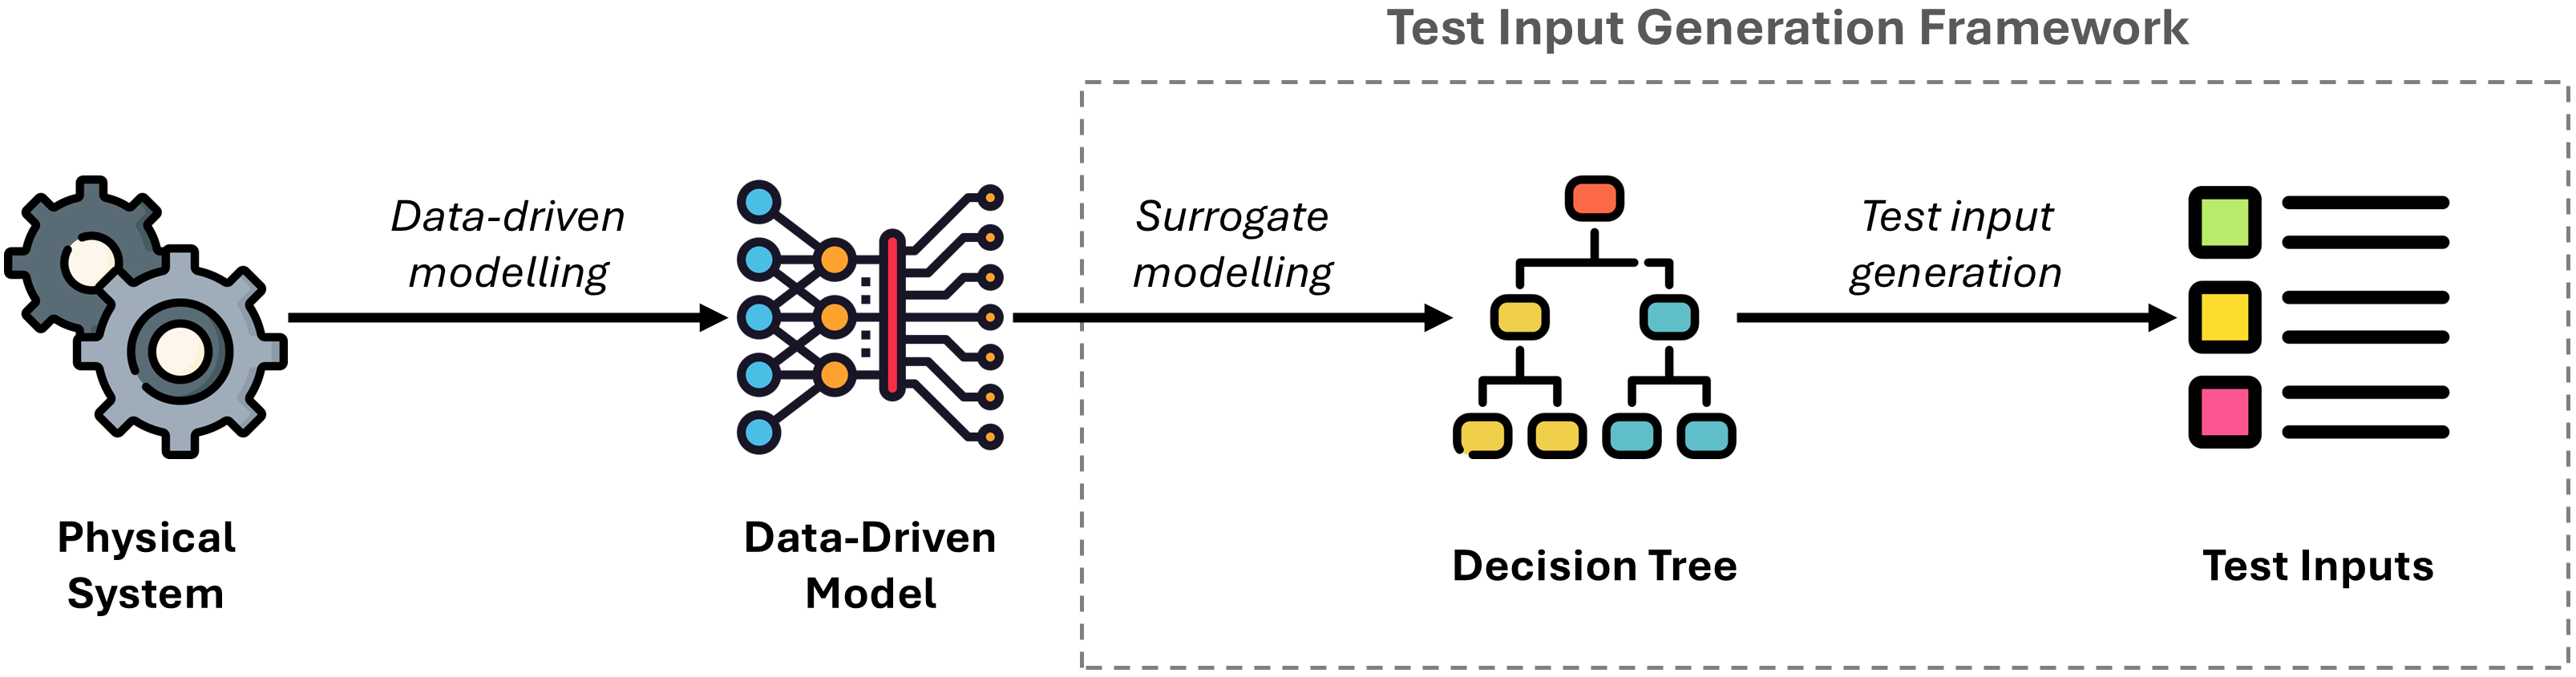
\includegraphics[width=\linewidth]{img/abstract}
\caption{Abstract workflow of our test input generation framework.}
\label{fig:abstract}
\end{figure}

Figure~\ref{fig:abstract} presents a high-level overview of the test input generation process within our framework. The framework produces test inputs based on the data-driven model of a CPS. This model is derived by applying a data-driven modelling process to the physical system. Once obtained, the model is fed into the framework, which employs a surrogate modelling approach to construct a decision tree. Subsequently, our test input generation method is applied to this decision tree to produce the final test inputs.

%% Significance of the Study
We compare the test inputs generated by our framework with those produced by four baseline methods, each employing different random sampling strategies. The evaluation considers three criteria: the effectiveness of the test inputs, the extent of input space coverage, and the distribution of inputs within the covered space. Simulation results indicate that, in the majority of test executions, our framework outperforms the baselines in generating challenging inputs that effectively push the SUT towards its operational limits. These results further demonstrate that the framework enables thorough exploration of the input space by generating inputs that span a broad range of values and are strategically dispersed according to user-defined criteria.

\paragraph{Contributions.} The main contributions of this paper are as follows:
\begin{itemize}
\item We present a systematic test input generation approach that exploits decision trees by applying equivalence class partitioning.
\item We propose a training mechanism that constructs a decision tree surrogate for any given data-driven model.
\item We empirically evaluate our framework, which combines surrogate modelling with test input generation, against baseline methods.
 \end{itemize}

%% Structure of Paper

The remainder of this paper is structured as follows. Section~\ref{sec:background} defines key terms and provides background on decision trees. Section~\ref{sec:related} reviews related work. Section~\ref{sec:method} introduces our method for generating test inputs from data-driven models. Section~\ref{sec:code} describes the software implementation, including the framework workflow and architecture. Section~\ref{sec:sim} outlines the simulation setup used to examine our research questions. Section~\ref{sec:res} analyses and evaluates the experimental results. Finally, Section~\ref{sec:end} concludes the paper.

Our test input generation framework, along with the experimental results, is publicly released under the BSD 3-Clause license on GitHub\footnote{\url{TODO}}.

\section{Background}
\label{sec:background}

This section explains the terminology used throughout this paper and reviews decision trees with an emphasis on their structure.

\subsection{Terminology}

This paper presents a framework for generating test inputs based on a data-driven model of a Cyber-Physical System~(CPS), as illustrated in Figure~\ref{fig:abstract}. A data-driven model is constructed primarily from data collected from the physical system and is used to represent its behaviour. Our proposed framework employs a surrogate modelling approach to build a decision tree from the data-driven model. The framework then uses the internal structure of this tree to generate test inputs. Surrogate models are simplified analytical representations that approximate the behaviour of complex, computationally intensive systems. Throughout this paper, we refer to the physical system being tested as the \textit{System Under Test}~(SUT). The data-driven model representing the SUT is termed the \textit{Model Under Test}~(MUT), treated as a black-box abstraction. This distinction separates the MUT from a decision tree model used specifically for test input generation. We also refer to such a decision tree model as the \textit{decision tree surrogate} or \textit{white-box surrogate}, as it approximates the MUT and provides a transparent structure for generating test inputs.

Let the input space of a data-driven model be defined as $\mathcal{X} = X_1 \times X_2 \times \dots \times X_n$, where each $X_i$ represents the domain of the $i$-th input feature. A \textit{test input} is a vector 
\begin{equation}
\mathbf{x} = (x_1, x_2, \dots, x_n) \in \mathcal{X},
\end{equation}
such that each $x_i \in X_i$ denotes the value assigned to the $i$-th feature, for $i \in \{1, 2, \dots, n\}$. Depending on the selected coverage criterion, these inputs may include normal, boundary, or invalid values. In contrast, a \textit{test case} consists of input values, execution conditions, and expected outcomes designed for a specific test objective~\cite{survey}. In the context of software testing, a \textit{test set} is a collection of individual test inputs used to evaluate a specific feature, function, or behaviour of the SUT. In this paper, we define a test set as
\begin{equation}
T = \{ \mathbf{x}^{(1)}, \mathbf{x}^{(2)}, \dots, \mathbf{x}^{(m)} \} \subseteq \mathcal{X},
\end{equation}
where each $\mathbf{x}^{(i)} \in \mathcal{X}$ is a test input, for $i \in \{1, 2, \dots, m\}$. The test set $T$ must satisfy a specified decision tree coverage criterion $C$, such that $C(T) = \texttt{true}$. Finally, \textit{test input generation} refers to the process of creating test inputs that effectively verify the behaviour of the SUT. 

\subsection{Decision Tree}

Decision trees are widely used non-parametric models in machine learning, particularly for classification and regression tasks. In classification, the goal is to assign a discrete label to an input instance, whereas regression involves predicting a continuous numerical value, often referred to as the target~\cite{mlbook}. When applied to classification problems, the model is known as a \textit{classification tree}; for regression tasks, it is called a \textit{regression tree}.

\begin{definition}[Decision Tree~\cite{swantje}]
A decision tree is a tree $T = (V, E)$, where $V$ is the set of nodes and $E \subseteq V \times V$ is the set of directed edges connecting them. The tree represents a predictor
\begin{equation*}
d: \mathcal{X} \rightarrow \mathcal{Y},
\end{equation*}
which maps a feature vector $\vb{x} \in \mathcal{X}$ to an output label $y \in \mathcal{Y}$. Each feature vector is defined as
\begin{equation*}
\vb{x} = (x^{(1)}, x^{(2)}, \ldots, x^{(D)}),
\end{equation*}
where $D$ is the number of measurable attributes. For classification tasks, ${y \in C}$, where $C = \{c_1, c_2, \dots, c_n\}$ is a finite set of $n$ class labels; for regression tasks, $y \in \mathbb{R}$.
\end{definition}

A decision tree learner constructs the tree using a training dataset of labeled examples, denoted as $\{(\vb x_i, y_i)\}^N_{i=1}$. The construction process involves recursively partitioning the dataset in distinct subsets based on some split values in the features. At each step, the learner evaluates all available features and their potential split values. The algorithm selects the features and split values that optimise a predefined heuristic measure. This process allows the tree to divide the input space into regions that correspond to different output labels.

A decision tree consists of three main structural components: nodes, branches, and paths~\cite{components}. \textit{Nodes} represent subsets of the training data and are categorised into two types: leaf nodes and inner nodes. Leaf nodes are defined as
\begin{equation}
V_L = \{ v \in V \mid \nexists\, (v, v') \in E \}, 
\end{equation}
i.e., nodes with no outgoing edges. Each leaf node $v \in V_L$ is assigned a label $y_v \in \mathcal{Y}$ based on the training data it contains and represents the final prediction after a sequence of decisions. The set of inner nodes is given by
\begin{equation}
V_I = V \setminus V_L.
\end{equation}
Each inner node $v \in V_I$ applies a split condition which partitions its data subset into disjoint child subsets based on feature values. The topmost inner node $v_{\text{root}} \in V_I$ is called the root node and represents the entire training dataset. \textit{Branches} correspond to edges $(v, v') \in E$. Each branch encodes one outcome of a split condition and directs the flow from a parent node $v \in V$ to a child node $v' \in V$. \textit{Paths} are sequences 
\begin{equation}
\pi = (v_0, e_1, v_1, \ldots, e_k, v_k),
\end{equation}
where ${v_0 = v_{\text{root}}}$, each edge ${e_i = (v_{i-1}, v_i) \in E}$ for ${i \in \{ 1, \dots, k \}}$, each intermediate node ${v_j \in V_I \setminus \{v_{\text{root}}\}}$ for $j \in \{ 1, \dots, k-1 \}$, and the final node $v_k \in V_L$. Each path encodes a decision rule that determines the prediction for a given input instance.

To make a prediction, the model starts at the root and follows the path determined by evaluating the split conditions at each inner node. Once a leaf is reached, the label associated with that leaf is returned.

In our approach, we employ binary decision trees to guide targeted test input generation. In a binary decision tree, each inner node branches into exactly two child nodes. This binary structure simplifies the decision-making process by evaluating a single condition at each node, such as whether a feature value is less than or greater than a specified threshold. Throughout this paper, we refer to the feature used for splitting at an inner node as the \textit{split feature}, and the corresponding threshold as the \textit{split threshold}. Each split condition is defined by a pair consisting of a split feature and a split threshold, which collectively determines the direction of traversal in the tree.

\paragraph{Hoeffding Tree.}

In this paper, we propose a method to train a decision tree surrogate from the MUT based on Hoeffding trees. This method is integrated into our test input generation framework, making it applicable to any data-driven models.

Hoeffding trees are an incremental decision tree learning algorithm designed specifically for mining data streams~\cite{hoeffding}. Unlike traditional decision tree learning methods, which require access to the entire dataset to construct a tree, Hoeffding trees operate in an online fashion. They update the tree incrementally using individual data instances as they arrive, without revisiting previously seen instances. This property makes them particularly suitable for environments where data is generated continuously and potentially without bound.

The key challenge in learning from data streams is making accurate split decisions at each node based on limited observations. Hoeffding trees address this challenge using a statistical tool known as the \textit{Hoeffding bound}. The Hoeffding bound provides a probabilistic guarantee that, with high probability, the feature selected for splitting at a node based on limited examples is the same as the one chosen using infinite examples. For a detailed explanation of the Hoeffding bound and its role in Hoeffding trees, see~\cite{hoeffding}.

A notable property of Hoeffding trees is their ability to produce decision trees that are asymptotically arbitrarily close to those generated by batch learners (i.e., learners that train on the entire dataset at once).  The probability that a Hoeffding tree and a conventional batch learner select different attributes at a node decreases exponentially with the number of examples. This implies that, given sufficient data, the structure of a Hoeffding tree converges to that of a tree trained on the complete dataset.

\section{Related Work}
\label{sec:related}

This section reviews existing research across two key domains relevant to our work: model-based testing of CPSs and validation methodologies for machine learning models (MLMs).

\paragraph{Model-based Testing of CPSs.}

Model-based testing approaches are commonly used to generate test cases from models that describe the architecture, design, or behaviour of a system, based on its specification~\cite{survey}. Deshmukh~et~al.~\cite{deshmukh} propose a Bayesian optimisation framework that constructs a surrogate model and uses an acquisition function to select test inputs. Menghi~et~al.~\cite{menghi} integrate falsification techniques with surrogate modelling to identify inputs that violate system requirements. Kosek and Gehrke~\cite{kosek} develop an anomaly detection method using artificial neural networks to identify rare data instances that deviate from expected patterns. Their neural network is trained on non-faulty data, resulting in a model that accurately approximates the behaviour of a correct system. Carter~et~al.~\cite{carter} present an automated testing framework that generates test cases using statistical models. These models simulate expected user-system interactions based on targeted usage scenarios. Araujo~et~al.~\cite{araujo} propose an approach that employs hybrid models to identify inputs which maximise the distance between test outputs and expected outputs. Such inputs are likely to drive the system into challenging states, increasing the chance of error detection. The hybrid models represent the desired behaviour of CPSs at a higher level of abstraction, making input generation feasible. Zhang~et~al.~\cite{zhang} apply formal methods to generate test cases for CPS conformance testing. Their approach uses differential dynamic logic to specify system behaviour and constructs a formal model from these specifications to derive test cases.

Although our proposed approach also relies on models to generate test inputs, the nature of these models differs from those used in~\cite{carter, araujo, zhang}. Our approach uses a model that approximates the behaviour of a physical system based on observed data. As such, it cannot reliably produce an expected system response for a given test input. Consequently, our method generates test inputs only, rather than complete test cases that include expected outcomes. In contrast, the models in~\cite{carter, araujo, zhang} represent the desired behaviour of a system, as defined by the system specification. By producing expected outcomes for given test inputs, these models support the generation of complete test cases. However, developing such models for CPSs is often challenging, as the process demands extensive domain expertise and is difficult to automate.

Our approach is more closely aligned with those proposed in \cite{deshmukh, menghi, kosek}. Similar to these studies, we build surrogate models from data-driven models to generate test inputs. However, these approaches use surrogate models to approximate system outputs and apply additional techniques to identify promising test inputs based on input-output pairs. By comparison, our method directly leverages the internal structure of the surrogate model to guide test input generation.

Cukic~et~al.~\cite{cukic} propose a method that automatically generates new test data from an existing set of test data using regression models. The new test data is statistically similar to the data in the original set, but sufficiently different to represent additional test cases. This represents a novel model-based testing approach compared to conventional methods used for CPSs. Rather than modelling system behaviour, as in our approach, their method builds a model from historical test data to generate new test data.

A recent survey~\cite{survey} by Sadri-Moshkenani~et~al.\@ provides a comprehensive overview of model-based test generation techniques for CPSs. The survey highlights the methodological characteristics of existing approaches and outlines open research challenges in scalability, coverage, and automation.

\paragraph{Validation Methodologies for MLMs.}

Recent studies explore property-driven validation techniques for machine learning models by employing surrogate models to guide test input generation. The work presented by Durelli~et~al.~\cite{durelli} is closely aligned with our research and shares several key similarities with the methodology described in this paper. In particular, Durelli et al.\@ propose a method that constructs a decision tree from the training data of an MLM and encodes tree traversal rules as logical formulae. These formulae are transformed into properties, which are used to systematically generate test suites. Analogous to our approach, their method derives test properties from the internal structure of a white-box surrogate model, eliminating the need for manual property specification. However, unlike our approach, their method does not leverage the statistics available at each node of the decision tree. As a result, test inputs are uniformly allocated across properties, without considering the varying significance of each property. Additionally, their approach only applies to classification models and cannot handle the continuous outputs typical of CPSs.

Sharma~et~al.~\cite{mlcheck} present \textsc{MLCheck}, a property-driven testing framework that includes a domain-specific language for property specification and a systematic test generation mechanism. Similar to our approach, \textsc{MLCheck} treats the MUT as a black-box and trains a white-box model (either a decision tree or a neural network) approximating the MUT by using its predictions. The white-box model in \textsc{MLCheck} is used to verify properties and extract counterexamples as test inputs for the original model. While effective, \textsc{MLCheck} requires testers to manually specify the properties under interest, which demands extensive domain knowledge. Furthermore, the framework focuses on property verification rather than using the surrogate model directly for test input generation, as is done in our approach.

Aggarwal~et~al.~\cite{fairness} propose a related approach that also involves constructing a decision-tree surrogate from the MUT. However, unlike our approach, their methodology applies dynamic symbolic execution to the tree to automatically generate test inputs.


\section{The Methodology}
\label{sec:method}

In this section, we first present a method for generating test inputs based on data-driven models by exploiting the internal structure of decision trees. To illustrate the approach, we provide a concrete example. Finally, we describe the procedure for training a decision tree surrogate from any given data-driven model. This allows our test input generation technique to be applied broadly across different model types.

Decision trees are employed as white-box surrogate models to guide the test input generation process due to their high interpretability. A surrogate model is a simplified analytical representation that approximates the behaviour of a complex, computationally intensive model. Interpretability, in this context, refers to the degree to which a human can understand the decision-making process of a machine learning model~\cite{interpretability}. Decision trees offer a high degree of interpretability through their hierarchical structure, which partitions the input space using simple, transparent decision rules. This transparency facilitates reasoning about the behaviour of the black-box MUT, thereby enabling the identification of informative test inputs.

The partitioning of input space by decision trees closely resembles the principle of equivalence class partitioning. Equivalence class partitioning is a testing technique that divides the input domain into a finite set of classes~\cite{ecp}. Each class represents a group of inputs that are processed similarly by the system. Instead of testing all possible inputs, representative values from each equivalence class are selected. This reduces the number of test cases significantly while maintaining broad coverage across input scenarios. This strategy is particularly effective for testing CPSs, which often exhibit large, continuous input spaces. By exploiting the structural properties of decision trees, we can infer equivalence classes over the input domain and systematically generate test inputs that are both diverse and representative.

\subsection{Test Input Generation}
\label{sec:test}

Our test input generation method consists of two main phases. The first phase involves extracting equivalence classes from a decision tree. The second phase samples test inputs based on these classes and a specified coverage criterion.

\begin{algorithm}
\caption{Extraction of Equivalence Classes from a Decision Tree}
\label{alg:eqclass}
\SetKwInOut{Input}{Input}
\SetKwInOut{Output}{Output}
\SetKwProg{Fn}{Function}{:}{}
\SetKwProg{Proc}{Procedure}{:}{}
\SetKwFunction{CollectPaths}{CollectAllPaths}
\SetKwFunction{InitClass}{InitEquivalenceClass}
\SetKwFunction{UpdateClass}{UpdateEquivalenceClass}

\Fn{\textnormal{ExtractEquivalenceClasses}$(T, \textnormal{specs})$}{
  \Input{Decision tree $T$; system specifications \textnormal{specs}}
  \Output{Set of equivalence classes $C$}

  $P \gets$ \CollectPaths{$T.\textnormal{root}$} \tcp*{Extract all root-to-leaf paths}
  $C \gets \emptyset$ \tcp*{Initialise class set}

  \ForEach{$\textnormal{path} \in P$}{
    $eq\_class \gets$ \InitClass{$\textnormal{specs}$}\;
    $parent \gets \textnormal{path}(0)$ \tcp*{Start at root}
    $m \gets \texttt{length} (\textnormal{path})$\;

    \For{$i \gets 1$ \KwTo $m$}{
      $node \gets \textnormal{path}(i)$ \;
      \UpdateClass{$eq\_class, parent, node$} \;
      $parent \gets node$ \;
    }

    $C \gets C \cup \{eq\_class\}$\;
  }

  \Return{$C$}
}

\vspace{0.5em}

\Proc{\textnormal{InitEquivalenceClass}$(\textnormal{specs})$}{
  \Input{System specifications \textnormal{specs}}
  \Output{Initialised equivalence class $eq\_class$}

  $F \gets \textnormal{specs(metadata).features}$ \tcp*{Extract feature list}

  \ForEach{$feature \in F$}{
    $eq\_class(feature) \gets$ \textbf{new} \textnormal{FeatureInterval}()\;
    $eq\_class(feature).\textnormal{max} \gets \textnormal{specs(feature).max}$\;
    $eq\_class(feature).\textnormal{max\_modified} \gets \textbf{false}$\;
    $eq\_class(feature).\textnormal{min} \gets \textnormal{specs(feature).min}$\;
    $eq\_class(feature).\textnormal{min\_modified} \gets \textbf{false}$\;
  }

  \Return{$eq\_class$}
}

\vspace{0.5em}

\Proc{\textnormal{UpdateEquivalenceClass}$(eq\_class, parent, node)$}{
  \Input{Equivalence class $eq\_class$; parent node $parent$; current node $node$}

  \eIf{$parent.\textnormal{child\_left} = node$}{
    $eq\_class(parent.\textnormal{feature}).\textnormal{max} \gets parent.\textnormal{threshold}$\;
    $eq\_class(parent.\textnormal{feature}).\textnormal{max\_modified} \gets \textbf{true}$\;
  }{
    $eq\_class(parent.\textnormal{feature}).\textnormal{min} \gets parent.\textnormal{threshold}$\;
    $eq\_class(parent.\textnormal{feature}).\textnormal{min\_modified} \gets \textbf{true}$\;
  }
}

\end{algorithm}

\begin{algorithm}
\caption{Collection of All Root-to-Leaf Paths in a Decision Tree~\cite{traversal}}
\label{alg:paths}
\SetKwInOut{Input}{Input}
\SetKwInOut{Output}{Output}
\SetKwProg{Fn}{Function}{:}{}
\SetKwProg{Proc}{Procedure}{:}{}
\SetKwFunction{CollectPaths}{CollectPaths}

\Fn{\textnormal{CollectAllPaths}$(\textnormal{root})$}{
  \Input{Root node of a decision tree $\textnormal{root}$}
  \Output{Set of all root-to-leaf paths $P$}

  $P \gets \emptyset$ \tcp*{Initialise path set}
  $path \gets \emptyset$ \tcp*{Temporary path container}

  \CollectPaths{$\textnormal{root}, path, P$} \tcp*{Recursive traversal}
  \Return{$P$}
}

\vspace{0.5em}

\Proc{\textnormal{CollectPaths}$(\textnormal{node}, path, P)$}{
  \Input{Current node $\textnormal{node}$; current path $path$; path set $P$}

  $path \gets path \cup \textnormal{node}$ \tcp*{Append current node}

  \eIf{$\textnormal{node.child\_left} = \textnormal{None} \land \textnormal{node.child\_right} = \textnormal{None}$}{
    $P \gets P \cup \{path\}$ \tcp*{Leaf node reached, store path}
  }{
    \CollectPaths{$\textnormal{node.child\_left}, path, P$} \tcp*{Explore left subtree}
    \CollectPaths{$\textnormal{node.child\_right}, path, P$} \tcp*{Explore right subtree}
  }

  $path.\textnormal{pop()}$ \tcp*{Backtrack for recursion}
}

\end{algorithm}

The process of extracting equivalence classes is described in Algorithm~\ref{alg:eqclass}, Lines 1–15. The algorithm first identifies all possible paths in the decision tree. Each path corresponds to a distinct equivalence class. For each path, the algorithm initialises a new class instance and traverses the associated nodes, updating the class intervals based on split thresholds and the direction of traversal.

The initialisation of an equivalence class instance is detailed in Algorithm~\ref{alg:eqclass}, Lines 16–25. The procedure begins by extracting input features from the system specification. For each feature, the class assigns value ranges based on the limits defined in the specification. Flags are also set to indicate that these ranges originate from the specification rather than the decision tree.

The procedure for updating an equivalence class instance is presented in Algorithm~\ref{alg:eqclass}, Lines 26–33. The procedure first determines whether the current node is the left or right child of its parent. This distinction reveals how the node satisfies the split condition at the parent node. Based on this, the procedure adjusts either the upper or lower bound of the relevant value range. The corresponding flag is set to indicate that the updated bound is derived from the decision tree. The split feature at the parent node determines which value range is affected during this update.

Algorithm~\ref{alg:paths}~\cite{traversal} illustrates how our method identifies all paths in a decision tree. The algorithm performs a recursive traversal of the decision tree, starting at the root and appending each visited node to the current path. Once a leaf node is reached, the complete path is stored. After exploring both the left and right subtrees, the function backtracks to search for alternative paths.

\paragraph{Decision Tree Coverage Criteria.}
Once equivalence classes are extracted from the decision tree, our method samples test inputs from them. To ensure the generation of effective inputs, we present two coverage criteria~\cite{durelli}. The first is \textit{Decision Tree Coverage}, defined as follows:
\begin{definition}[Decision Tree Coverage (DTC)]
\label{def:dtc}
A test set is DTC-adequate if the execution of its inputs causes the model to traverse every path from the root to each leaf node at least once.
\end{definition}
In essence, a DTC-adequate test set ensures that the decision tree predicts every possible label at least once. This guarantees that all equivalence classes are covered during testing.

The second criterion is \textit{Boundary Value Analysis}, defined as follows:
\begin{definition}[Boundary Value Analysis (BVA)]
\label{def:bva}
A test set is BVA-adequate if its inputs are sampled from the boundaries of all equivalence classes, specifically those boundaries derived from the structure of the decision tree.
\end{definition}
BVA complements equivalence class partitioning by targeting the edges of input domains. In this context, boundaries derived from the tree structure correspond to the split conditions of the decision tree. These split features and thresholds are considered informative for predicting the output label of an input instance. Consequently, even small perturbations in input values near these boundaries can lead to different outputs from the decision tree. Such boundary regions in the input space are often sensitive and may reveal weaknesses in the behaviour of the system. By testing inputs in these regions, BVA can help identify potential vulnerabilities in the SUT.

\begin{algorithm}[htbp]
\caption{Sample Generation from an Equivalence Class Guided by Decision Tree Coverage}
\label{alg:dtc}
\SetKwInOut{Input}{Input}
\SetKwInOut{Output}{Output}
\SetKwProg{Fn}{Function}{:}{}
\SetKwFunction{GenSamples}{GenerateRandomSamples}
\SetKwFor{ForEach}{for each}{do}{end}
\SetKwComment{Comment}{\tcp{}}{}

\Fn{\textnormal{GenerateDTCSamples}$(eq\_class, n)$}{
  \Input{Equivalence class $eq\_class$; number of test inputs $n$}
  \Output{Set of sample vectors $I$}

  $I \gets \emptyset$ \Comment*[r]{Initialise set of sample vectors}

  \ForEach{$feature\_range \in eq\_class$}{
    $min \gets feature\_range.\textnormal{min}$\;
    $max \gets feature\_range.\textnormal{max}$\;

    \eIf{$feature\_range.\textnormal{min\_modified} = \textbf{true}$}{
      $samples \gets$ \GenSamples{$(min,\ max],\ n$}\;
      $I \gets I \cup \{samples\}$\;
    }{
      $samples \gets$ \GenSamples{$[min,\ max],\ n$}\;
      $I \gets I \cup \{samples\}$\;
    }
  }

  \Return{$I$}
}
\end{algorithm}

\begin{algorithm}[htbp]
\caption{Sample Generation from an Equivalence Class Guided by Boundary Value Analysis}
\label{alg:bva}
\SetKwInOut{Input}{Input}
\SetKwInOut{Output}{Output}
\SetKwProg{Fn}{Function}{:}{}
\SetKwFunction{GenSamples}{GenerateRandomSamples}
\SetKwFor{ForEach}{for each}{do}{end}
\SetKwComment{Comment}{\tcp{}}{}


\Fn{\textnormal{GenerateBVASamples}$(eq\_class, \epsilon, n)$}{
  \Input{Equivalence class $eq\_class$; boundary neighbourhood size $\epsilon$; number of test inputs $n$}
  \Output{Set of sample vectors $I$}

  $I \gets \emptyset$ \Comment*[r]{Initialise set of sample vectors}

  \ForEach{$feature\_range \in eq\_class$}{
    $min \gets feature\_range.\textnormal{min}$\;
    $max \gets feature\_range.\textnormal{max}$\;

    \uIf{$feature\_range.\textnormal{max\_modified} = \textbf{true}$ \textbf{and} $feature\_range.\textnormal{min\_modified} = \textbf{true}$}{
      $k_1 \gets \lceil \frac{n}{2} \rceil$\;
      $k_2 \gets \lfloor \frac{n}{2} \rfloor$\;
      $samples_1 \gets$ \GenSamples{$[max - \epsilon,\ max + \epsilon],\ k_1$}\;
      $samples_2 \gets$ \GenSamples{$[min - \epsilon,\ min + \epsilon],\ k_2$}\;
      $I \gets I \cup \{samples_1 \cup samples_2\}$\;
    }
    \uElseIf{$feature\_range.\textnormal{max\_modified} = \textbf{true}$}{
      $samples \gets$ \GenSamples{$[max - \epsilon,\ max + \epsilon],\ n$}\;
      $I \gets I \cup  \{samples\}$\;
    }
    \uElseIf{$feature\_range.\textnormal{min\_modified} = \textbf{true}$}{
      $samples \gets$ \GenSamples{$[min - \epsilon,\ min + \epsilon],\ n$}\;
      $I \gets I \cup \{samples$\}\;
    }
    \Else{
      $samples \gets$ \GenSamples{$[min,\ max],\ n$}\;
      $I \gets I \cup \{samples\}$\;
    }
  }

  \Return{$I$}
}
\end{algorithm}

\begin{algorithm}[htbp]
\caption{Generate Test Inputs from an Equivalence Class}
\label{alg:testinput}
\SetKwInOut{Input}{Input}
\SetKwInOut{Output}{Output}
\SetKwProg{Fn}{Function}{:}{}
\SetKwFor{For}{for}{do}{}
\SetKwComment{Comment}{\tcp{}}{}

\Fn{GenerateTestInputs($I$)}{
  \Input{Set of $n$ sample vectors $I = \{I_1, I_2, \ldots, I_n\}$, where each $I_j$ contains $m$ samples of feature $j$}
  \Output{Set of $m$ test inputs $T = \{t_1, t_2, \ldots, t_m\}$, where each $t_i$ contains $n$ feature values} 

  $T \gets \emptyset$ \Comment*[r]{Initialise set of test inputs}
  $m \gets \texttt{length}(I_1)$ \Comment*[r]{All sample vectors have equal length}

  \For{$i \gets 1$ \KwTo $m$}{
    $t \gets \emptyset$ \Comment*[r]{Initialise a test input}

    \For{$j \gets 1$ \KwTo $n$}{
      $t \gets t \cup \{I_j(i)\}$ \Comment*[r]{Select $i$-th sample from $j$-th sample vector}
    }

    $T \gets T \cup \{t\}$\;
  }

  \Return{$S$}
}
\end{algorithm}

\paragraph{}Following the extraction of equivalence classes (Algorithm~\ref{alg:eqclass}), the second phase of our test input generation method focuses on sampling test inputs based on a specified coverage criterion. This phase utilises the equivalence classes derived from decision tree paths to guide the sampling process.

Algorithms~\ref{alg:dtc} and \ref{alg:bva} describe two sampling strategies: Decision Tree Coverage (DTC) and Boundary Value Analysis (BVA), respectively. Both algorithms produce a set of sample vectors for a given equivalence class. Each vector contains values sampled according to the feature-specific value range defined by the class. These vectors are then combined to form complete test inputs by aligning values at corresponding positions across all vectors.

We first describe the DTC-based sampling procedure. The algorithm samples input values from a given equivalence class, assuming that each decision tree node applies a split condition of the form \lstinline{split_feature <= split_threshold}. For each feature in the class, the algorithm examines its value range and determines whether the lower bound is derived from the tree structure. If so, values are randomly sampled from the left-open interval $(min, max]$, where $min$ and $max$ denote the lower and upper bounds of the value range. Otherwise, sampling is performed over the closed interval $[min, max]$. These intervals are designed to ensure that the resulting test inputs follow the decision tree path corresponding to the equivalence class, as defined by DTC. Each set of sampled values is stored in a sample vector and added to the set of sample vectors.

Next, we describe the BVA-based sampling procedure. The algorithm samples input values around the boundaries of a given equivalence class. For each feature in the class, the algorithm checks whether the bounds are derived from the decision tree. If both bounds are derived from the tree, values are sampled around both the upper and lower boundaries. If only one bound is derived, sampling occurs around that boundary. This condition ensures that values are distributed around decision boundaries, consistent with BVA principles. If neither bound originates from the tree, values are sampled from the global feature range defined in the specification. Although these bounds are not critical for boundary testing, sampling is still necessary to ensure that each test input includes a value for every feature. Each set of sampled values is stored in a sample vector and added to the set of sample vectors.

The set of sample vectors generated by Algorithms~\ref{alg:dtc} and \ref{alg:bva} serve as input to Algorithm~\ref{alg:testinput}, which constructs complete test inputs. Each test input is formed by aggregating values at the same index across all sample vectors, resulting in a tuple that includes one value per feature. To generate a DTC-adequate or BVA-adequate test set, the sampling process (Algorithm~\ref{alg:dtc} or \ref{alg:bva}) and the combination process (Algorithm~\ref{alg:testinput}) are repeated for each equivalence class extracted from the decision tree.

Our method allocates a variable number of test inputs to each equivalence class. The allocation is based on the number of training examples that reach the leaf node corresponding to the path from which the equivalence class is derived. We define an equivalence class as dominant if its corresponding leaf node contains more training examples than others. Dominant classes represent regions of the input space that are frequently accessed during system operation. Therefore, it is important to sample more test inputs from these regions to ensure reliable performance under typical conditions. Conversely, equivalence classes associated with leaf nodes containing fewer training examples represent less commonly accessed regions of the input space. Sampling more test inputs from these regions can help reveal hidden errors and improve system robustness under edge-case conditions. To support both testing objectives, we propose two allocation strategies. The tester may select the appropriate strategy based on the test requirements and objectives.

In the first strategy, dominant equivalence classes receive more test inputs:
\begin{definition}[Proportional Allocation Function]
\label{def:prop}
Let $S = \{s_1, s_2, \ldots, s_m\}$ be a set of integers, where each $s_j$ denotes the number of training examples reaching the leaf node of path $j$. Let $\left[ x \right]$ denote the Banker's rounding function~\cite{banker}, which rounds $x$ to the nearest integer; if $x$ is exactly halfway between two integers, it is rounded to the nearest even integer. Let $t$ be the total number of test inputs to be generated. The number of test inputs $n_j$ allocated to equivalence class $j$ is computed as:
\begin{equation*}
n_j = \left[ t \cdot \frac{s_j}{\sum_{i=1}^{m} s_i} \right] \qquad \forall\ 1 \leq j \leq m .
\end{equation*}
\end{definition}

In the second strategy, less dominant equivalence classes receive more test inputs:
\begin{definition}[Inverse Allocation Function]
\label{def:inverse}
Let $N = \{n_1, n_2, \ldots, n_l\}$ be a sorted set of integers such that $n_1 \leq n_2 \leq \ldots \leq n_l$, where each $n_j$ denotes the number of test inputs allocated to equivalence class $j$, as computed using Equation~\eqref{eq:prop}. The number of test inputs $m_j$ assigned to equivalence class $j$ is defined as:
\begin{equation*}
m_j = n_{l - (j - 1)} .
\end{equation*}
\end{definition}

\subsection{A Motivating Example}

\begin{figure}
\centering
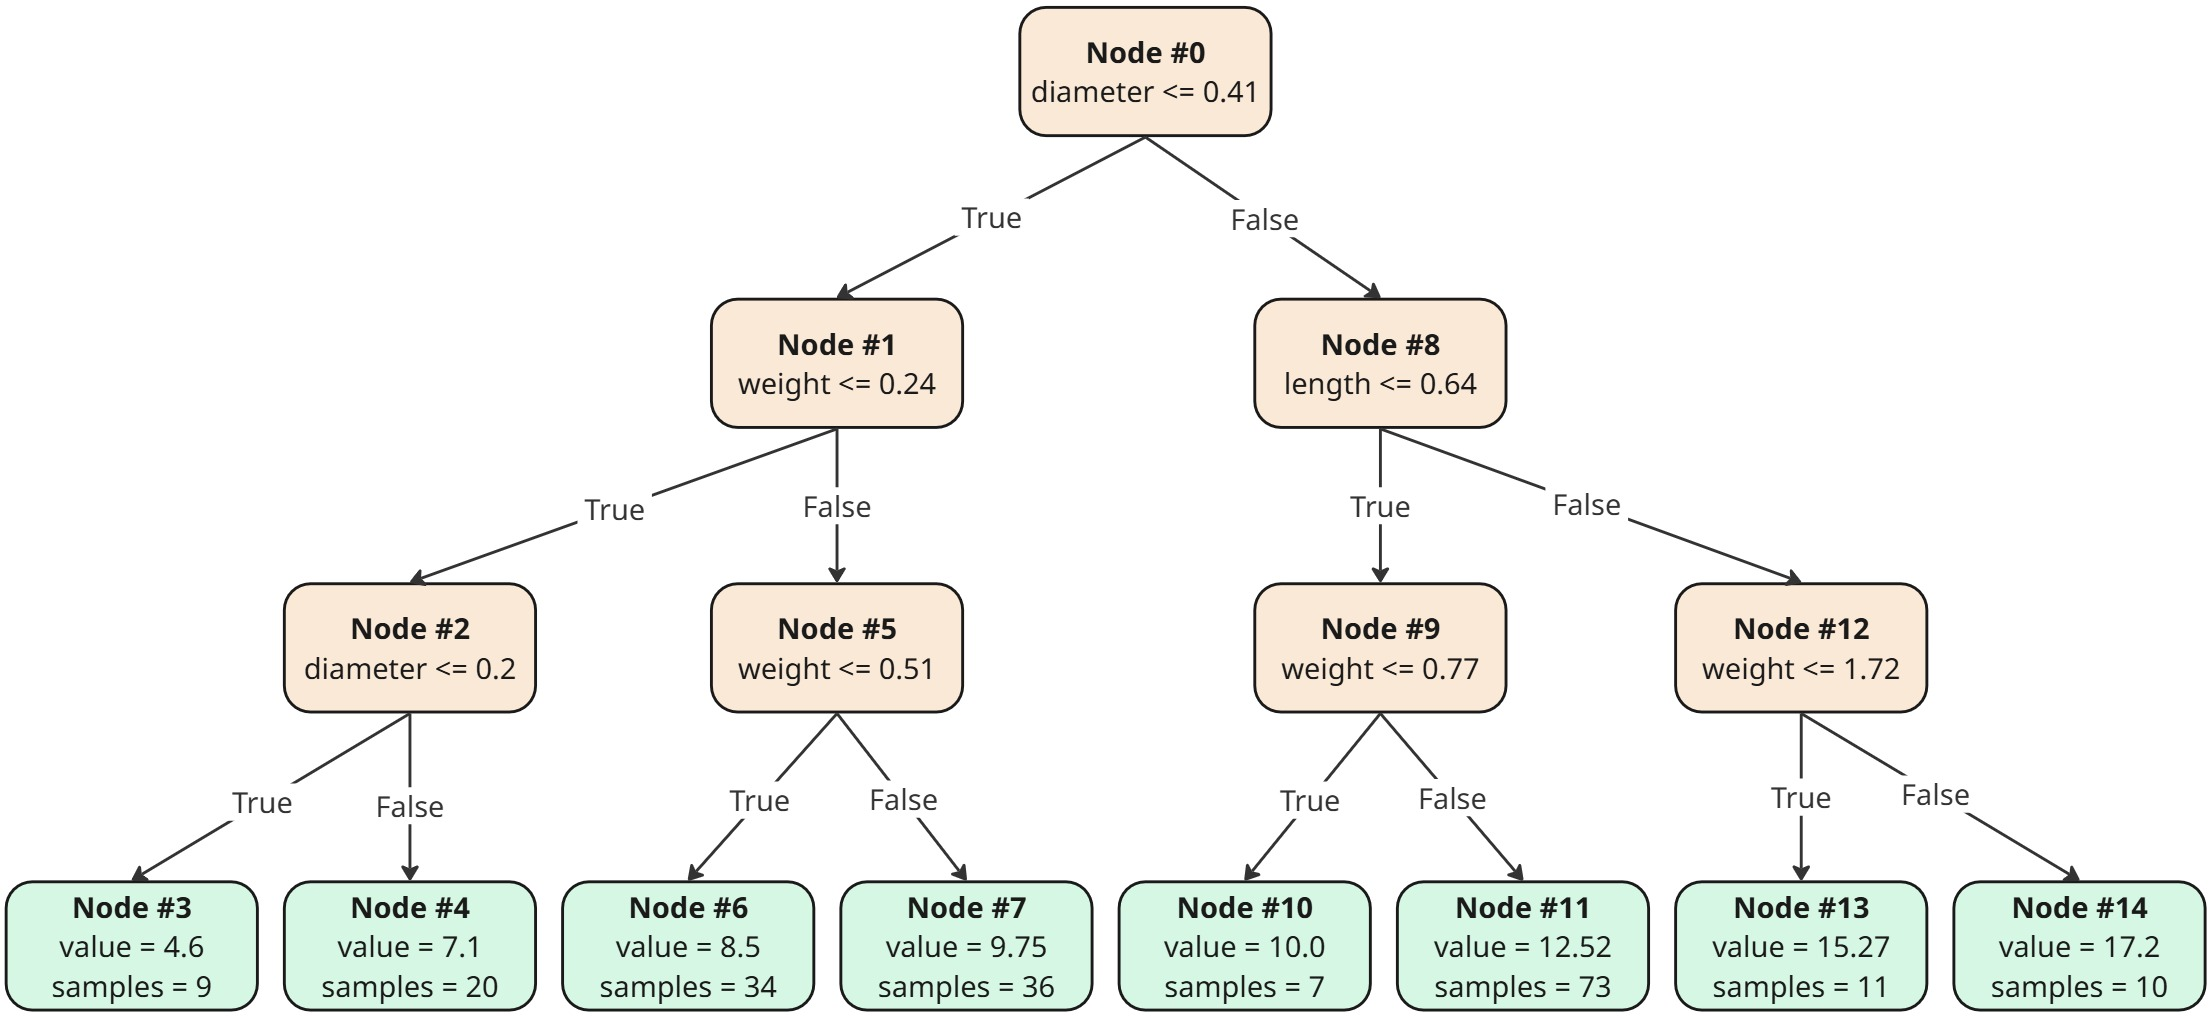
\includegraphics[width=\linewidth]{img/abalonetree}
\caption{Decision tree generated from the Abalone dataset. Leaf nodes are highlighted in green and inner nodes in orange. Node \#0 represents the root. Each leaf node displays the predicted age of the abalone and the number of training samples that reached it during model training.}
\label{fig:abalonetree}
\end{figure}

We demonstrate our test input generation approach using a decision tree constructed from the Abalone dataset~\cite{abalone}. Instead of training a model on system-specific input and output data, we use the Abalone dataset for its simplicity. This dataset contains physical measurements of abalones, and the task is to predict their age based on these measurements. The relevant features are:
\begin{itemize}
\item Length -- the longest shell measurement (in mm)
\item Diameter -- measured perpendicular to the length (in mm)
\item Weight -- the total weight of the abalone (in grams)
\end{itemize}
Figure~\ref{fig:abalonetree} presents the decision tree generated from this dataset. The tree consists of 15 nodes: eight leaf nodes (highlighted in green) and seven inner nodes (highlighted in orange). The topmost inner nodes, labeled as node \#0, is the root node. Each inner node defines a split condition of the form \lstinline{split_feature <= split_threshold}. Input instances that satisfy this condition are directed to the left child node for further evaluation; otherwise, they proceed to the right child node. Each leaf node contains a predicted age value for the abalone, along with a sample count indicating how many training examples reached that node during training.

\begin{table}
\caption{Equivalence classes extracted from the Abalone decision tree. The final two columns indicate the number of test inputs to be generated for each class, calculated according to Definitions~\ref{def:prop} and \ref{def:inverse}, respectively. The total number of test inputs is set to $t = 100$. The other columns specify the upper and lower bounds of the value ranges for each feature within each equivalence class. Bounds highlighted in bold are externally specified by the tester.}
\label{tab:eqclass}
\begin{tabular}{ccccccccc}\toprule
 \multirow{2}{*}{Class} & \multicolumn{2}{c}{Length} & \multicolumn{2}{c}{Diameter}  & \multicolumn{2}{c}{Weight}& \multirow{2}{*}{\# Test Inputs (Def.~\ref{def:prop})}& \multirow{2}{*}{\# Test Inputs (Def.~\ref{def:inverse})}
\\\cmidrule(lr){2-3}\cmidrule(lr){4-5}\cmidrule(lr){6-7}
      & $min$  & $max$ & $min$    & $max$  & $min$ & $max$\\\midrule
1    & \textbf{0.17} & \textbf{0.73} & \textbf{0.13} & 0.2              & \textbf{0.03} & 0.24 & 4 & 36\\
2 & \textbf{0.17} & \textbf{0.73} & 0.2                   & 0.41            & \textbf{0.03} & 0.24 & 10& 6\\
3 & \textbf{0.17} & \textbf{0.73} & \textbf{0.13} & 0.41               & 0.24 & 0.51              & 17& 5\\
4 & \textbf{0.17} & \textbf{0.73} & \textbf{0.13} & 0.41                & 0.51 & \textbf{2.55} & 18& 4\\
5 & \textbf{0.17} & 0.64              & 0.41                 & \textbf{0.58} & \textbf{0.03} & 0.77 & 4 & 18\\
6 & \textbf{0.17} & 0.64              & 0.41                & \textbf{0.58} & 0.77 & \textbf{2.55} & 36 & 4\\
7 & 0.64 & \textbf{0.73}              & 0.41                 & \textbf{0.58} & \textbf{0.03} & 1.72 & 6 & 10\\
8   & 0.64 & \textbf{0.73}            & 0.41                 & \textbf{0.58} & 1.72 & \textbf{2.55} & 5& 17 \\\bottomrule
\end{tabular}
\end{table}

When applying our proposed method to the Abalone decision tree, the algorithm first traverses the tree to identify all distinct paths. From each path, it extracts an equivalence class, as described in Algorithm~\ref{alg:eqclass}. Since the tree contains eight distinct paths, the method yields eight equivalence classes. Table~\ref{tab:eqclass} presents these extracted equivalence classes. In the table, equivalence classes are listed top-down, corresponding to tree paths ordered from left to right. Each equivalence class consists of three value ranges, one for each feature in the Abalone dataset. For each range, a lower and upper bound is specified, denoted as $min$ and $max$ in the table. These bounds are derived by analyzing the split conditions of internal nodes along each path. Some features may not appear in any split condition for a given path. For example, the feature Length is not used in the leftmost path. In other cases, only one bound (either upper or lower) can be determined. For instance, in the leftmost path, only upper bounds for Diameter and Weight can be extracted. When a bound cannot be inferred from the tree traversal, it is taken from the specification provided by the tester. These bounds are highlighted in bold in the table. The final two columns in Table~\ref{tab:eqclass} show the number of test inputs to be generated for each equivalence class, computed using two different approaches outlined in Definitions~\ref{def:prop} and \ref{def:inverse}, respectively. For this computation, we set the total number of test inputs to be generated as $t = 100$.

\begin{table}
\caption{Feature intervals used for sampling test inputs generated under Decision Tree Coverage (DTC) and Boundary Value Analysis (BVA). For BVA, a neighbourhood size of $\epsilon = 0.05$ is applied to each boundary value.}
\label{tab:interval}
\begin{tabular}{ccccccccc}\toprule
Coverage Criterion & Length & Diameter  &Weight \\\midrule
DTC    &  $[0.17, 0.73]$ & $[0.13, 0.20]$ & $[0.03, 0.24]$ \\
BVA   & $[0.17, 0.73]$ & $[0.15, 0.25]$ & $[0.19, 0.29]$ \\\bottomrule
\end{tabular}
\end{table}

The next phase of our method involves sampling test inputs from the equivalence classes based on a specified coverage criterion. For clarity, we illustrate this process using only Equivalence Class 1, as shown in Table~\ref{tab:eqclass}. Table~\ref{tab:interval} lists the feature intervals used for sampling test inputs, as described in Algorithms~\ref{alg:dtc} and \ref{alg:bva}. The intervals vary depending on the chosen coverage criterion: Decision Tree Coverage (DTC) or Boundary Value Analysis (BVA). Intervals generated under DTC are designed to ensure that the sampled values, when used as test inputs, follow the tree path associated with Equivalence Class 1. In contrast, intervals derived from BVA target values within an $\epsilon$-neighbourhood of all boundary values extracted from the same path. For this example, we set $\epsilon = 0.05$. For features whose boundary values are externally specified by the tester, the corresponding intervals follow the DTC-based structure. These boundaries are considered less critical for testing, as they do not appear along the relevant tree path. In Table~\ref{tab:interval}, this applies to the feature Length.

To generate four test inputs for Equivalence Class 1, we sample four values from each DTC interval listed in Table~\ref{tab:interval}. Following the procedure described in Algorithm~\ref{alg:dtc}, we construct three sample vectors, each corresponding to a specific feature:

\begin{equation*}
\begin{aligned}
& \text{Length}:&[0.63, 0.40, 0.39, 0.66] , \\
& \text{Diameter}:&[0.16, 0.17, 0.16, 0.14] , \\
& \text{Weight}:&[0.08, 0.05, 0.18, 0.20] . \\
\end{aligned}
\end{equation*}

Each vector contains four independently sampled values from its corresponding feature interval. By combining values across these vectors, as described in Algorithm~\ref{alg:testinput}, we generate the following test inputs:

\begin{equation*}
\begin{aligned}
& \text{Test Input \#1}: (0.63, 0.16, 0.08) , \\
& \text{Test Input \#2}: (0.40, 0.17, 0.05) , \\
& \text{Test Input \#3}: (0.39, 0.16, 0.18) , \\
& \text{Test Input \#4}: (0.66, 0.14, 0.20) . \\
\end{aligned}
\end{equation*}

Each test input is a tuple consisting of values for Length, Diameter, and Weight, respectively. The same procedure can be applied to generate test inputs using intervals derived from BVA, as outlined in Algorithm~\ref{alg:bva}.

\subsection{Surrogate Modelling}
\label{sec:surrogate}

\begin{figure}
\centering
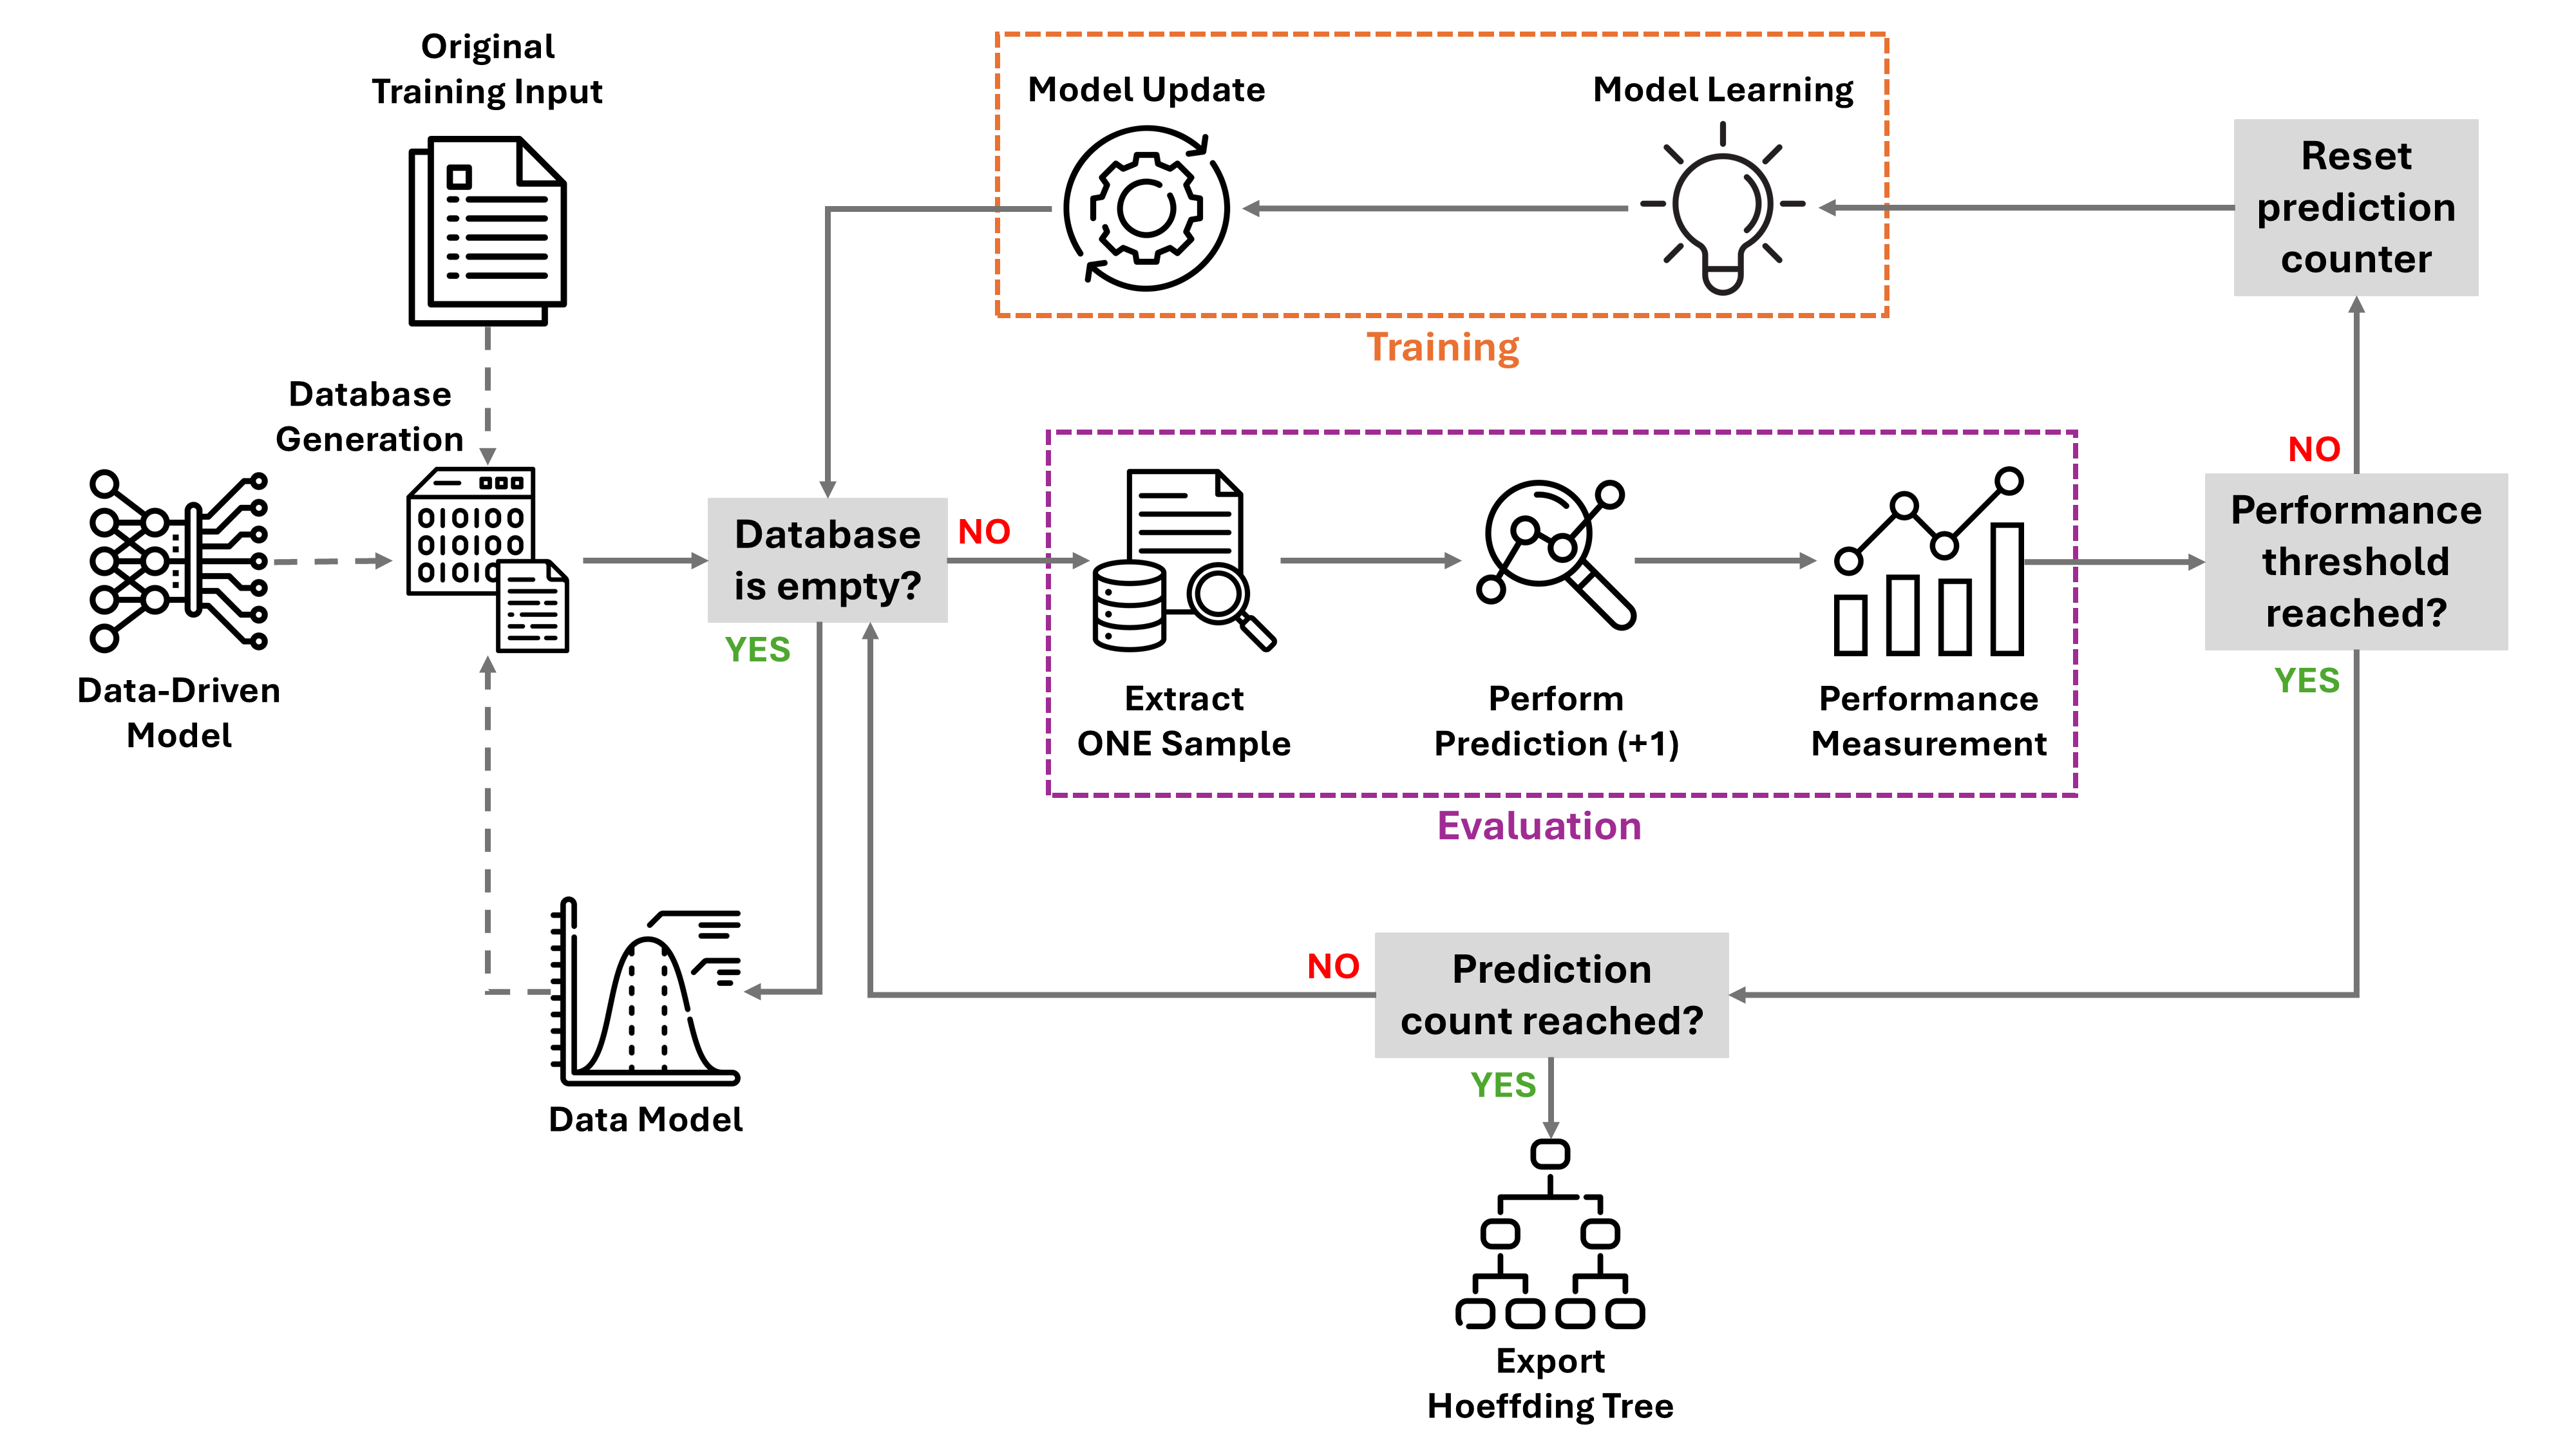
\includegraphics[width=\linewidth]{img/surrogate}
\caption{Workflow for constructing a decision-tree surrogate from a data-driven model.}
\label{fig:surrogate}
\end{figure}

To ensure our test input generation method is applicable to any data-driven model, we propose a technique for constructing a decision-tree surrogate using incrementally learned Hoeffding Trees. Surrogate models are simplified analytical representations that approximate the behaviour of complex, computationally intensive systems. Our goal is not to replicate the predictions of the black-box MUT with high fidelity. Instead, we aim to optimise split features and thresholds in the surrogate decision tree by analysing the input-output behaviour of the MUT. These splits define input regions represented by equivalence classes, which serve as the basis for generating effective test inputs.

Figure~\ref{fig:surrogate} illustrates the workflow for generating a decision-tree surrogate from a data-driven model. The process begins by constructing a dynamic database that pairs original training inputs with outputs produced by the MUT. This database is continuously updated with new data points. Inputs are generated by a data model, and outputs are obtained by querying the MUT. The data model ensures that generated inputs follow the same distribution as the original training data. To build the data model, we use empirical distributions for discrete-valued features and kernel density estimation (KDE) for continuous-valued features~\cite{dectext}. An empirical distribution represents the probability of each value in a dataset. KDE estimates the probability density function (PDF) based on the original training data, using kernels as weighting functions~\cite{kde}. For our KDE implementation, we use the commonly adopted Gaussian kernel. The estimated PDF is computed as:
\begin{equation}
f(x) = \frac{1}{m}\sum^m_j\left[ \frac{1}{\sqrt{2\pi\sigma}}e^{-\left(\frac{x-\mu_j}{2\sigma}\right)^2} \right] ,
\end{equation}
where:
\begin{itemize}
\setlength{\itemindent}{1em}
\item[$m$] \hspace*{0.5em}is the number of training examples,
\item[$\mu_j$] \hspace*{0.5em}is the value of the feature for the $j$-th example,
\item[$\sigma$] \hspace*{0.5em}is the width of the Gaussian kernel.
\end{itemize}
As the number of training examples increases, the estimated PDF converges to the true distribution. When data is scarce, the method yields near-Gaussian estimates.

Each data point in the database is sequentially passed to the Hoeffding Tree for processing. Initially, the tree is empty, i.e., it contains no nodes or branches, until the first data point triggers its construction. The tree generates a prediction based on the input. This prediction is then compared to the output from the MUT to assess the performance of the current tree. If the performance falls below a predefined threshold, the prediction counter is reset, and the current sample is used to update the tree. If the threshold is met, the algorithm checks whether the required number of correct predictions has been achieved. If so, the Hoeffding Tree is finalised; otherwise, the process continues with new data points. The resulting Hoeffding Tree serves as a white-box surrogate model that approximates the behaviour of the original data-driven model and guides the test input generation process.

This approach offers significant flexibility and control. Due to the incremental nature of Hoeffding Trees, the training and evaluation phases can be managed independently, allowing for precise tuning toward the desired performance. Furthermore, the number of training examples used to construct the surrogate can be adjusted to meet the predefined performance threshold.

\paragraph{Why Hoeffding Trees?}
Our surrogate modelling approach involves training a decision tree using examples drawn from an open-ended data stream. This is made possible by models capable of generating an infinite sequence of input-output pairs, which continuously populate the training database. Our goal is to construct a decision tree that meets a predefined performance threshold, based on a specified data-driven model. To achieve this, we require a learning method that operates continuously, examining new examples as they arrive without discarding valuable information. The method must fully utilise all available training data and continue learning until the performance criterion is satisfied. This strategy ensures low computational cost while adapting to data-driven models of varying complexity. For simpler models, fewer training examples may suffice to meet the desired performance, while more complex models typically demand larger datasets. These requirements are well addressed by incremental learning algorithms. Among them, we choose Hoeffding Trees due to their suitability for streaming data and strong theoretical guarantees~\cite{hoeffding}. As an incremental learner, Hoeffding Trees produce models similar to those obtained through batch learning on the same dataset. Additionally, they are robust to the order of incoming examples, maintaining consistent performance regardless of input sequence. Hoeffding Trees process each example only once and do not require storing data from the stream. They operate in time proportional to the number of features and require only a single pass over the data. As a result, they scale efficiently to extremely large or even infinite datasets with minimal computational overhead. These properties make Hoeffding Trees a well-suited choice for our surrogate modelling method.

\section{Implemention}
\label{sec:code}

We implement the approach described in Section~\ref{sec:method} as a test input generation framework. This section outlines the main parameters of the framework, its workflow, and the underlying software architecture.

The framework is written in Python (v3.10.11) and comprises approximately 1500 lines of code. We use the \lstinline{river}\footnote{\url{https://riverml.xyz/0.22.0}} library (v0.22.0) for incremental training of the decision tree surrogate. For kernel density estimation, used to construct the data model in the surrogate modeling process, we rely on the \lstinline{scikit-learn}\footnote{\url{https://scikit-learn.org/1.6}} library (v1.6.1).

\begin{table}
\caption{Parameters of our test input generation framework}
\label{tab:parameters}
\begin{tabular}{lll}\toprule
Parameter & Type & Explanation \\\midrule
\lstinline{model}                    &   $M: \vec{X} \rightarrow \vec{Y}$ & data-driven MUT  \\
\lstinline{train_set}                 &  $\vec{X}$ & training dataset used for MUT \\
\lstinline{specification_file}     &  JSON & input specification file  \\
\lstinline{coverage_criterion}  &  \{\textit{dtc}, \textit{bva}\}& decision tree coverage criterion  \\
\lstinline{n_test_inputs}           & integer & total number of test inputs  \\
\lstinline{test_allocation}        &  \{\textit{proportional}, \textit{inverse}\} & test input allocation strategy   \\
\lstinline{epsilon}                   &  float & boundary neighbourhood size for BVA  \\\bottomrule
\end{tabular}
\end{table}

Table~\ref{tab:parameters} summarises the main parameters of the framework. The core input is a data-driven model representing the SUT, provided via the \lstinline{model} parameter. This model must implement a \lstinline{predict()} function that returns an output for a given input instance. This functionality is essential for generating training examples used to train the decision tree surrogate. The training dataset used to train the data-driven model must also be supplied, via the \lstinline{train_set} parameter. This dataset is required both for constructing the data model and for training the surrogate. The \lstinline{specification_file} parameter refers to a JSON file that defines the input parameters of the SUT, including metadata such as minimum and maximum values, as well as data types. The \lstinline{coverage_criterion} parameter specifies the decision tree coverage criterion used for test input generation, as detailed in Section~\ref{sec:test}. The total number of test inputs to be generated is set via \lstinline{n_test_inputs}. The \lstinline{test_allocation} parameter defines how test inputs are distributed across equivalence classes, either proportionally or inversely, also described in Section~\ref{sec:test}. Finally, the \lstinline{epsilon} parameter controls the neighbourhood size around each boundary value used in Boundary Value Analysis (BVA).

\subsection{Workflow}

\begin{figure}
\centering
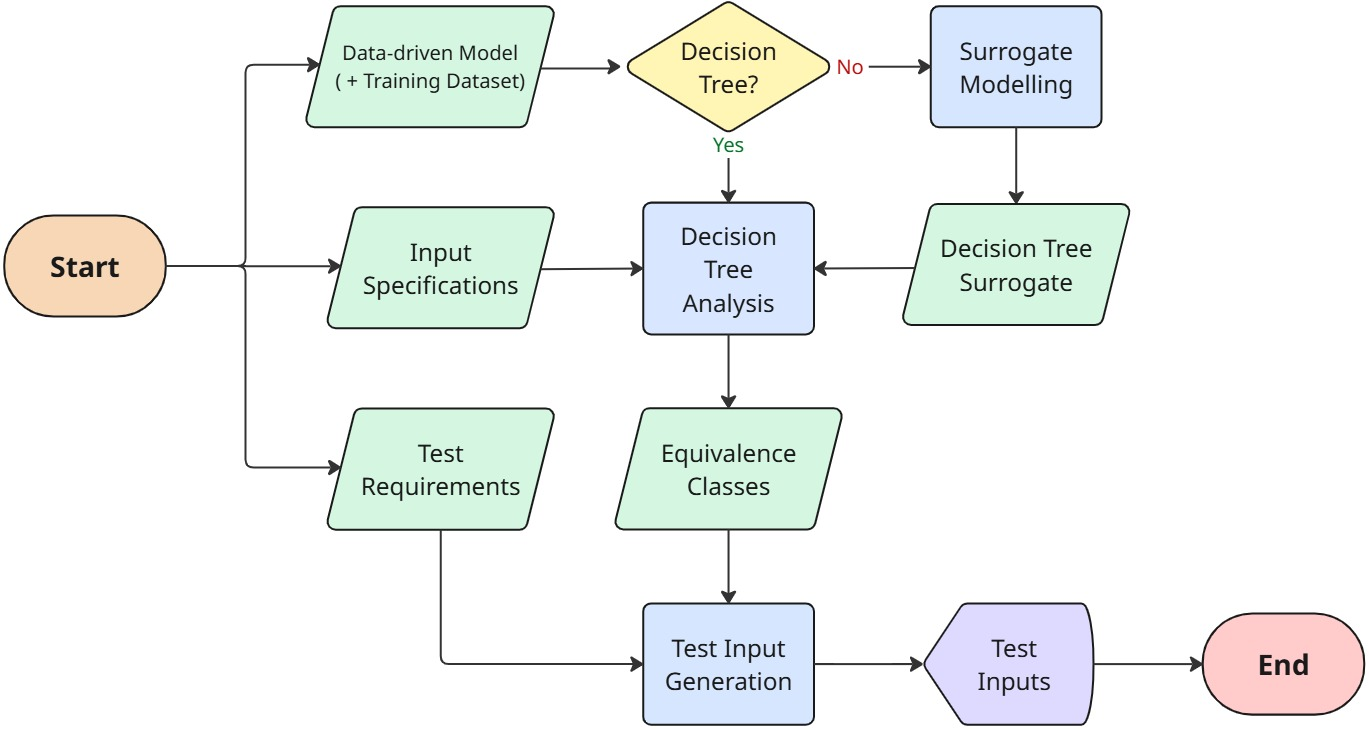
\includegraphics[scale=0.3]{img/workflow}
\caption{Detailed workflow of our test input generation framework.}
\label{fig:workflow}
\end{figure}

Figure~\ref{fig:workflow} provides a detailed overview of the workflow used in our test input generation framework. The process begins with the framework receiving a data-driven model that describes the behaviour of the SUT. If the model is not a decision tree, the tester must also supply the training dataset used to construct the model. In addition, the tester provides a specification file describing the input parameters of the SUT, including their value ranges and data types. The tester must also specify the test requirements by assigning values to the parameters \lstinline{coverage_criterion}, \mbox{\lstinline{n_test_inputs},} \lstinline{test_allocation}, and \lstinline{epsilon}, as listed in Table~\ref{tab:parameters}. The framework first checks whether the provided model is a decision tree. If not, it applies the surrogate modelling technique described in Section~\ref{sec:surrogate} to construct a decision tree surrogate. If the model is already a decision tree, it is used directly for test input generation. Next, the framework analyses the internal structure of the decision tree and uses the input specifications to identify equivalence classes, as outlined in Section~\ref{sec:test}. Based on the specified test requirements, the framework applies the method from Section~\ref{sec:test} to generate test inputs from these equivalence classes. The resulting test inputs are then produced as output.

\subsection{Software Architecture}

\begin{figure}
\centering
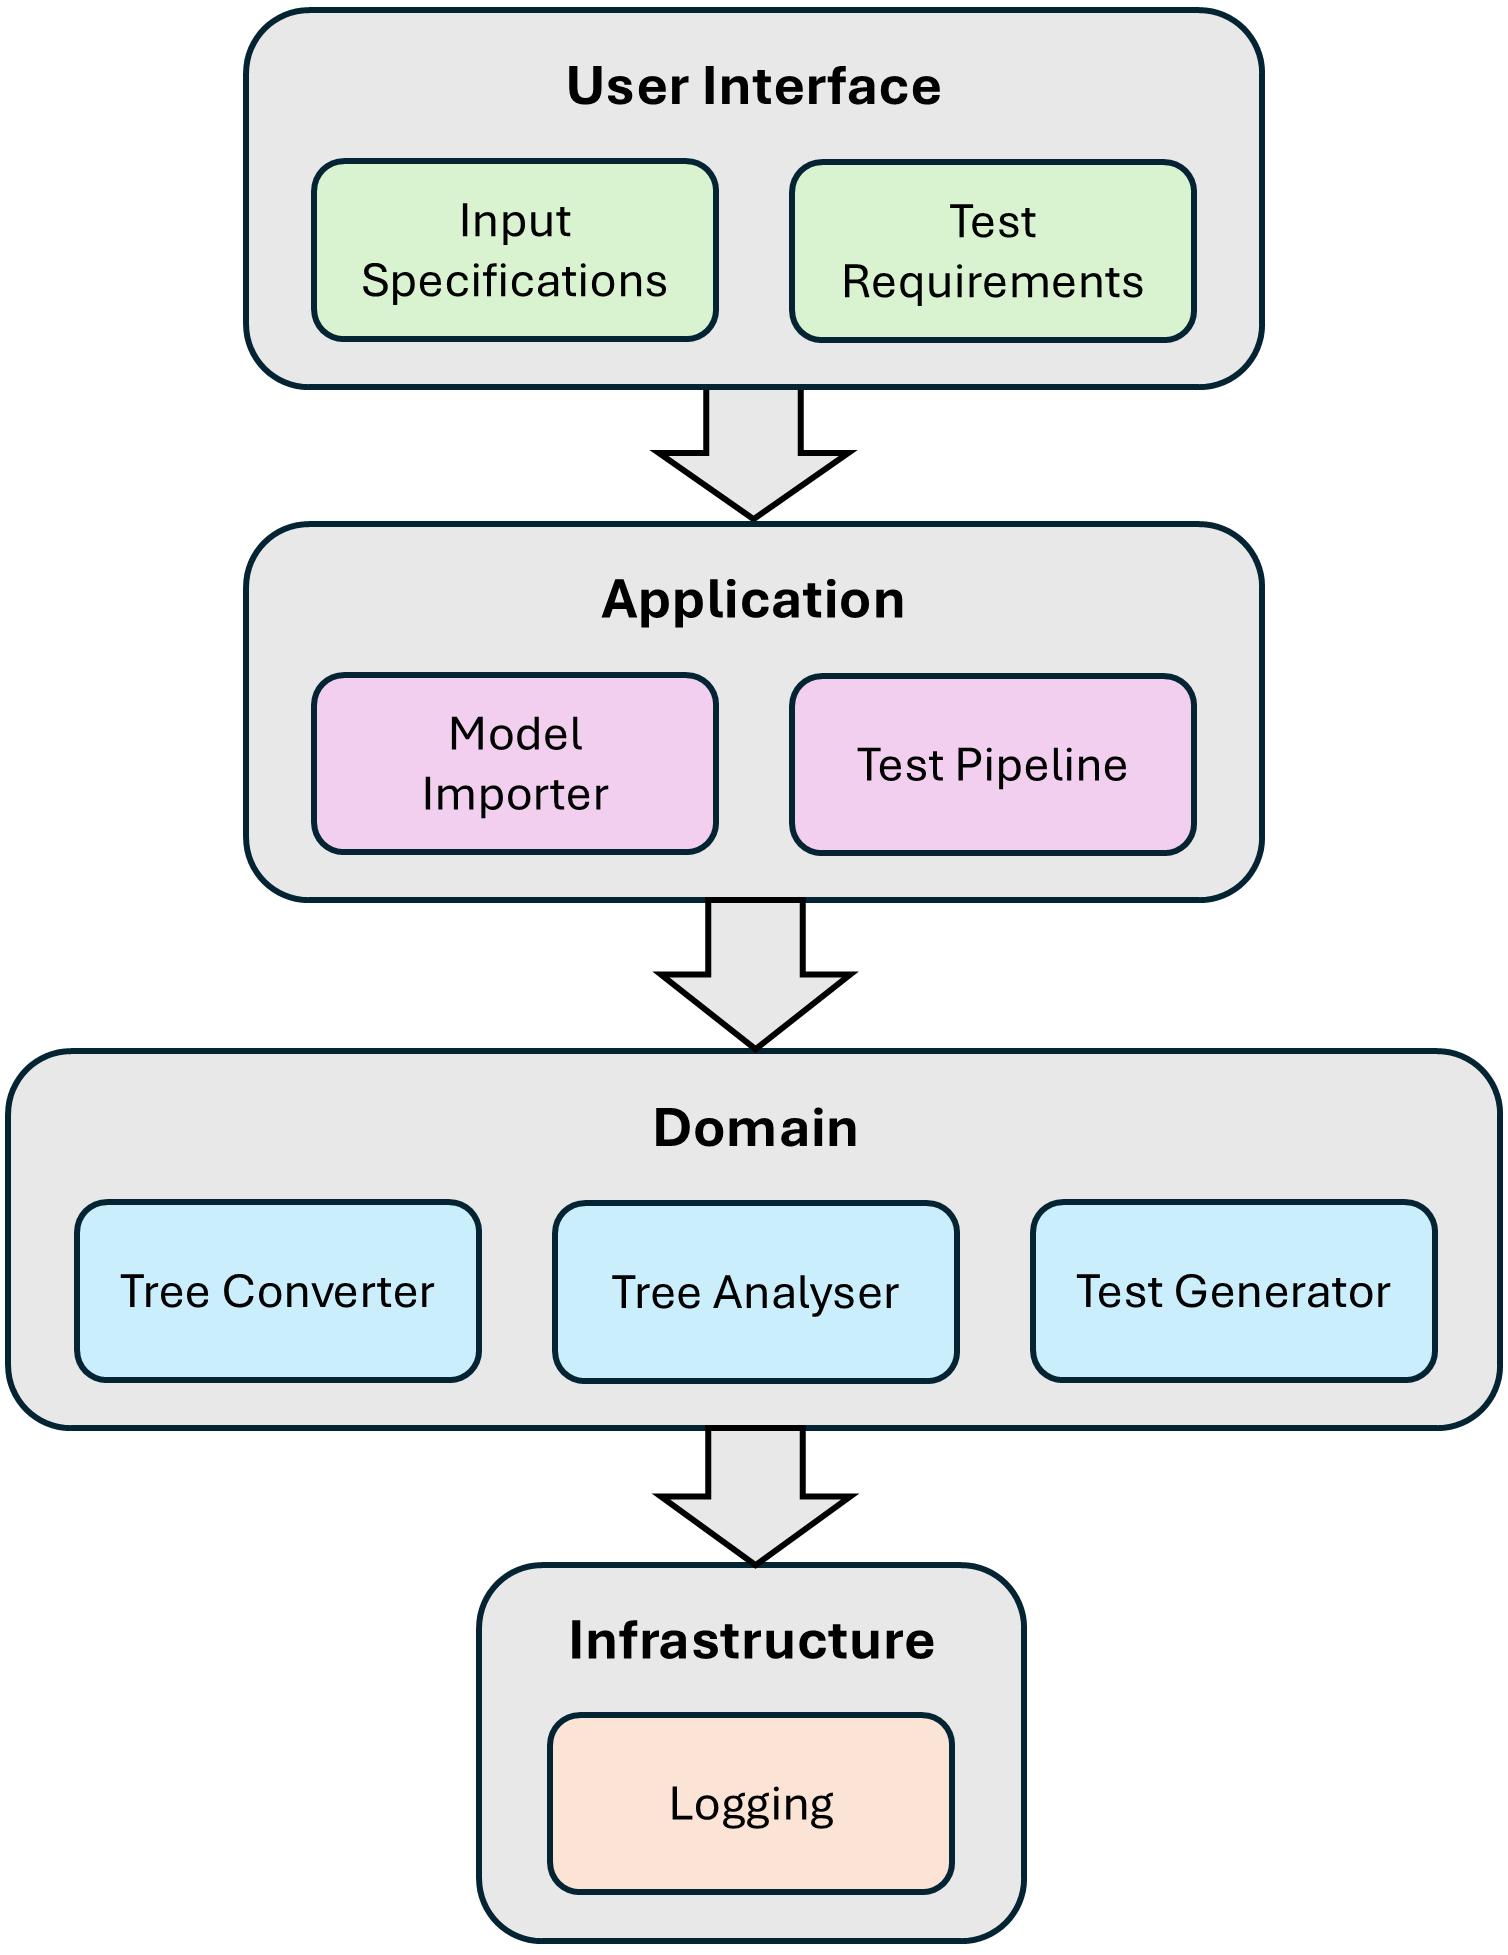
\includegraphics[scale=0.6]{img/architecture}
\caption{Software architecture of our test input generation framework.}
\label{fig:architecture}
\end{figure}

The software architecture of our test input generation framework is structured into multiple layers, each fulfilling a specific role. These layers follow a top-down hierarchy, where higher layers depend on services provided by lower ones, but not the other way around~\cite{layer}. Modules within a layer may interact with other modules in the same layer or with those below, while remaining independent of any above. This separation of concerns promotes modularity, simplifies development and testing, and improves maintainability.

Figure~\ref{fig:architecture} illustrates the layered architecture of our framework. At the top is the User Interface Layer, responsible for managing user inputs. This layer consists of two modules. The Input Specifications module converts a specification file into a format compatible with the framework. The file contains metadata describing the input parameters of the SUT. Similarly, the Test Requirements module translates the test requirements into a format suitable for further processing. Beneath this lies the Application Layer, which integrates the data-driven model and defines the overall workflow. This layer comprises two modules. The Model Importer module provides an interface for importing a data-driven model of the SUT. The module also implements a wrapper function that invokes the \lstinline{predict()} method of the model. This wrapper function enables modules in the lower layer to easily retrieve model predictions for given input instances. The Test Pipeline module manages execution and assigns relevant tasks to each module within the Domain Layer. The Domain Layer forms the core of the framework and performs its primary functions. This layer consists of three modules. The Tree Converter module applies the surrogate modelling technique described in Section~\ref{sec:surrogate} to construct a decision tree surrogate when the input model is not already a decision tree. The Tree Analyser module examines the structure of a decision tree to identify equivalence classes. The Test Generator module is responsible for producing test inputs. Finally, the Infrastructure Layer provides technical support for the Domain Layer. The layer includes the Logging module, which records the surrogate model, equivalence classes, and generated test inputs. In addition, the module logs operations throughout execution of the framework for the purpose of monitoring progress and facilitating debugging.

\begin{figure}
\centering
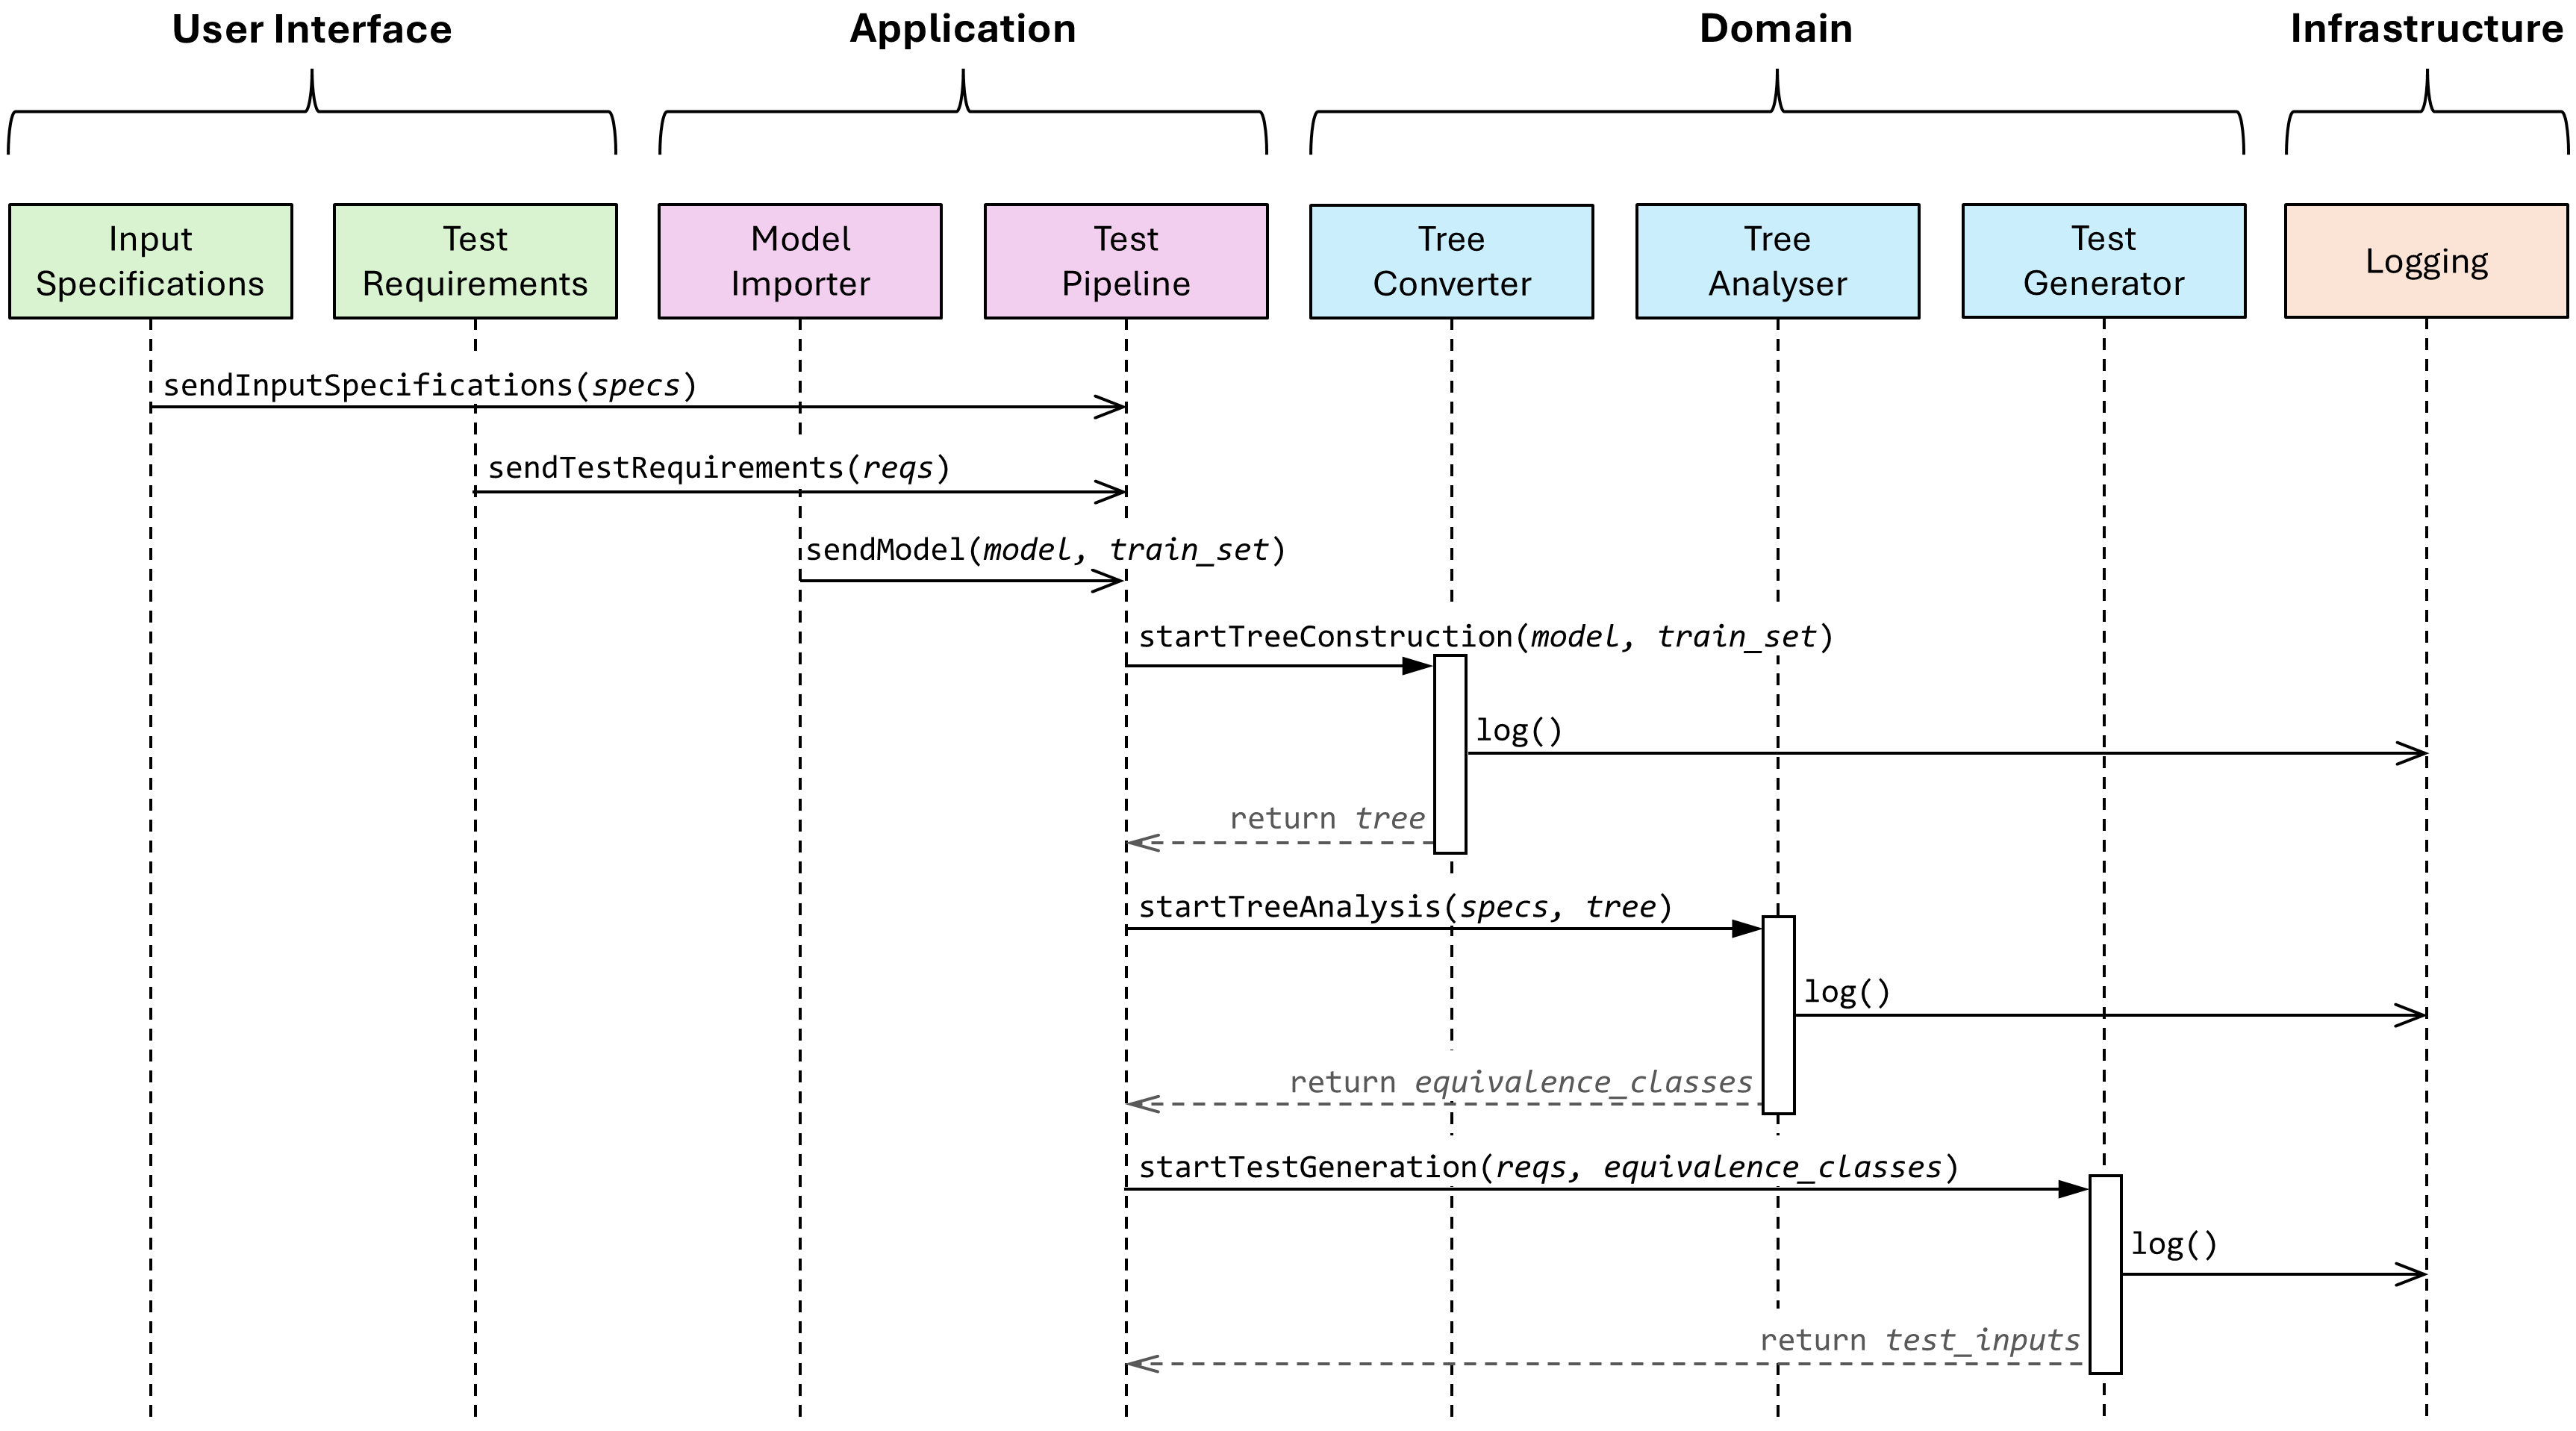
\includegraphics[width=\linewidth]{img/msc}
\caption{Message sequence chart illustrating the interactions between modules across different layers of the framework.}
\label{fig:msc}
\end{figure}

Figure~\ref{fig:msc} presents a message sequence chart that illustrates interactions between modules across the various layers of the framework. The process begins when the Input Specifications module receives input specifications from the tester and processes them. The formatted data is forwarded to the Test Pipeline module for further handling. Similarly, the Test Requirements module receives and processes the test requirements before passing the formatted output to the Test Pipeline module. Upon receiving a data-driven model of the SUT and its corresponding training data, the Model Importer module transfers both to the Test Pipeline module. The Test Pipeline module is responsible for coordinating the overall workflow of the framework. The module first determines whether the data-driven model is a decision tree. If so, it signals the Tree Converter module to begin the surrogate modelling process, providing the model and training data as inputs. Once the surrogate model has been constructed, the Test Pipeline module initiates the tree analysis phase. The Tree Analyser module receives the decision tree and input specifications, performs structural analysis, and extracts equivalence classes. Upon completion, the Tree Analyser module returns the equivalence classes to the Test Pipeline module. These classes, along with the test requirements, are passed to the Test Generator module, which generates the test inputs. The surrogate modelling, tree analysis, and test generation processes are each logged using the infrastructure provided by the Logging module. Once complete, the Test Generator module returns the test inputs to the Test Pipeline module. Finally, the Test Pipeline module delivers the generated test inputs to the tester.

\section{Simulation}
\label{sec:sim}

We aim to evaluate the effectiveness of the test inputs generated by our framework in assessing the performance of the SUT. To achieve this, we compare our test inputs with those produced by four baseline methods. These baselines rely on various random sampling strategies, either from the input space of the SUT or from the training data of a data-driven model. In addition to effectiveness, we assess the input space coverage achieved by our approach. This is done by comparing the distribution of our test inputs with those generated by the baseline methods. To guide our evaluation, we design a series of simulations to address the following Research Questions (RQs):
\begin{enumerate}[align=left]
\item[\textbf{RQ1:}] How effective are test inputs generated by our framework without surrogate modelling (i.e., using a decision tree as the input model) compared to those produced by baseline methods?
\item[\textbf{RQ2:}] How effective are test inputs generated by our framework with surrogate modelling (i.e., using a decision tree as the input model) compared to those produced by baseline methods?
\item[\textbf{RQ3:}] How extensively do our test inputs explore the input space compared to baseline methods, and how are they distributed within that space?
\end{enumerate}

In the following section, we present the hypotheses used to investigate these questions. We then describe the simulation setup used to conduct the experiments. Finally, we review the evaluation metrics used to measure the performance of our framework.

\subsection{Hypotheses Formulation}

We hypothesise that our framework is capable of generating effective test inputs from data-driven models. This prediction is based on the use of decision tree surrogates within the framework to construct equivalence classes by analysing their internal structure and decision-making information. These classes define subsets of the input space of the SUT, from which representative values are sampled for test input generation. By partitioning the input space, the number of required test inputs is significantly reduced while maintaining comprehensive coverage. Furthermore, the framework applies decision tree coverage criteria and test allocation strategies to guide the sampling process. These mechanisms help generate test inputs that satisfy diverse testing requirements and objectives.

Based on this prediction and the research questions, we formulate the following hypotheses:
\begin{enumerate}[align=left]
  \item[\textbf{H1:}] Test inputs generated by our framework without surrogate modelling are more effective than those produced by baseline methods.
  \item[\textbf{H2:}] Test inputs generated by our framework with surrogate modelling are more effective than those produced by baseline methods.
  \item[\textbf{H3:}] Test inputs generated by our framework achieve greater input space coverage compared to those generated by baseline methods.
  \item[\textbf{H4:}] Test inputs generated by our framework follow a distribution that reflects the proposed test allocation strategies.
\end{enumerate}

\subsection{Evaluation Metrics}

To assess the effectiveness of test inputs generated by different methods, we use the F\textsubscript{1} score for classification models and the Mean Absolute Error~(MAE) for regression models. Both metrics are widely accepted standards for assessing model performance in their respective domains. In the context of our evaluation, if a model $M$ performs worse on test inputs generated by one approach $A_1$ than on those produced by another approach $A_2$, then $A_1$ is considered more effective than $A_2$~\cite{durelli}.

Formally, for classification models:
\begin{definition}[Effectiveness Based on F\textsubscript{1} Score]
\label{def:claeff}
Given a classification model $M$ and a set of test inputs $T$, we denote the F\textsubscript{1} score obtained by evaluating $M$ on $T$ as $F_1(M(T))$. Consequently,
\begin{equation*}
F_1(M(T_1)) < F_1(M(T_2))
\end{equation*}
indicates that $T_1$ is more effective than $T_2$, as it reveals a larger number of misclassifications by $M$.
\end{definition}

For regression models:
\begin{definition}[Effectiveness Based on MAE]
\label{def:regeff}
Given a regression model $M$ and a set of test inputs $T$, we denote the MAE obtained by evaluating $M$ on $T$ as $E(M(T))$. Consequently,
\begin{equation*}
E(M(T_1)) > E(M(T_2))
\end{equation*}
indicates that $T_1$ is more effective than $T_2$, as it reveals a higher average prediction error in $M$.
\end{definition}

Separate definitions of effectiveness are required for classification and regression models due to the nature of their evaluation metrics. A higher F\textsubscript{1} score reflects better predictive accuracy in classification tasks, whereas a lower MAE indicates higher accuracy in regression tasks.

We evaluate input space coverage by computing the volume of the \textit{Minimum Bounding Box}~(MBB) for each set of test inputs. The volume of an MBB provides a measure of how extensively a given set explores the input space. By comparing these volumes across different test input generation strategies, we assess the relative effectiveness of each method in spanning the input space. Formally, the MBB and its volume are defined as follows:
\begin{definition}[Volume of a Minimum Bounding Box~\cite{mbb}]
\label{def:mbb}
Let $X = \{x_1, x_2, \dots, x_m\} \subset \mathbb{R}^n$ be a set of $m$ test inputs in an $n$-dimensional space. Each test input $x_i = (x_{i1}, x_{i2}, \dots, x_{in})$ represents values across $n$ features. The \textit{Minimum Bounding Box} is the smallest axis-aligned hyperrectangle (i.e., with edges parallel to the coordinate axes) that contains all test inputs in $X$. Its \textit{volume} $V$ is computed as:
\begin{equation*}
V = \prod_{j=1}^{n} \left( \max_{1 \leq i \leq m} x_{ij} - \min_{1 \leq i \leq m} x_{ij} \right).
\end{equation*}
\end{definition}

Even when the input space is broadly covered, test inputs may still be sparsely distributed, leaving gaps that result in untested regions. To quantify this distribution, we compute the \textit{Coefficient of Variation}~(CV) for each set of test inputs and compare the values across different test input generation methods. CV measures the relative variability in a distribution with respect to its mean~\cite{cv}. A low CV indicates low variability around the mean, suggesting that test inputs are more uniformly spread but may be tightly clustered and concentrated. In contrast, a high CV reflects greater variability, meaning test inputs are unevenly distributed and more widely scattered across different regions of the input space. For this evaluation, the CV is computed from the standard deviation and mean of the pairwise \textit{Mahalanobis distances} between all test inputs in a given set. We formally define the Mahalanobis-based CV as follows:

\begin{definition}[Mahalanobis-Based Coefficient of Variation]
\label{def:cv}
Let $X = \{x_1, x_2, \dots, x_m\} \subset \mathbb{R}^n$ be a set of $m$ test inputs, where each input $x_i = (x_{i1}, x_{i2}, \dots, x_{in})$ consists of values across $n$ features. Let $D_M(x_i, x_j)$ denote the Mahalanobis distance between inputs $x_i$ and $x_j$ in the multivariate input space.
The mean pairwise Mahalanobis distance is given by:
\begin{equation*}
\bar{D} = \frac{2}{m(m-1)} \sum_{1 \leq i < j \leq m} D_M(x_i, x_j).
\end{equation*}
The corresponding variance is:
\begin{equation*}
\sigma^2 = \frac{2}{m(m-1)} \sum_{1 \leq i < j \leq m} \left( D_M(x_i, x_j) - \bar{D} \right)^2.
\end{equation*}
The standard deviation is then:
\begin{equation*}
\sigma = \sqrt{\sigma^2}.
\end{equation*}
Finally, the Coefficient of Variation is defined as:
\begin{equation*}
\text{CV} = \frac{\sigma}{\bar{D}}.
\end{equation*}
\end{definition}

\subsection{Setup}
\label{sec:setup}
% when describing setup -> generalize by mentioning comparing performance metric

The primary objective of the simulation is to evaluate the effectiveness of the test inputs generated by our framework. To this end, we conduct two distinct simulations: one in which the framework generates test inputs without surrogate modelling, and another in which surrogate modelling is employed prior to test input generation. In addition, we generate test inputs using four baseline methods and compare their effectiveness against those from our framework using a defined set of metrics. We further analyse the coverage and distribution of the test inputs across the input space using a separate set of metrics and provide a comprehensive comparison between our framework and the baseline methods.

\begin{table}
\centering
\begin{minipage}{0.45\textwidth}
\captionof{table}{Overview of the datasets used for classification \\ tasks in the simulation.}
\label{tab:cladata}
\footnotesize
\begin{tabular}{llll}\toprule
Dataset                               & Features & Instances  & Classes \\\midrule
Banknote Authentication    &  4 & 1372 & 2  \\
Breast Cancer Wisconsin    &  30 & 569 & 2 \\
Dry Bean                            &  16 & 13611 & 7 \\
Iranian Churn                    &  13 & 3150 & 2 \\
Iris                              &  4 & 150 & 3 \\
Mammography  & 6 & 11183 & 2 \\
Phishing Websites    &  30 & 11055 & 2 \\
Pima Indians Diabetes   &  8 & 2768 & 2 \\
Seeds                           &  7 & 210 & 3 \\
Sonar, Mines vs. Rocks       &  60 & 208 & 2 \\
Vertebral Column    &  6 & 310 & 3 \\
Wireless Localisation    &  7 & 2000 & 4 \\\bottomrule
\end{tabular}
\end{minipage}
\hfill
\begin{minipage}{0.45\textwidth}
\captionof{table}{Overview of the datasets used for regression \\ tasks in the simulation.}
\label{tab:regdata}
\footnotesize
\begin{tabular}{lll}\toprule
Dataset                               & Features & Instances   \\\midrule
Appliances Energy    &  27 & 19735   \\
Body Fat       &  14 & 252  \\
Combined Cycle Power Plant  & 4 & 9568  \\
Concrete Strength    &  8 & 1030  \\
Forest Fires    &  29 & 517  \\
Liver Disorders         &  5 & 345  \\
Parkinsons Telemonitoring          &  19 & 5875  \\
Real Estate Valuation    &  6 & 414  \\
Superconductor Temperature   &  81 & 21263  \\
Seoul Bike Sharing Demand    &  15 & 8760  \\
Wind Power                           &  8 & 43800  \\
Wind Speed    &  7 & 5638  \\\bottomrule
\end{tabular}
\end{minipage}
\end{table}

\paragraph{Datasets.} To construct the data-driven input MUTs used in our framework, we selected 24 diverse datasets, including both classification and regression tasks. These datasets are sourced from the UCI Machine Learning Repository\footnote{\url{https://archive.ics.uci.edu/datasets}} and the online data science platform Kaggle\footnote{\url{https://www.kaggle.com/datasets}}. Table~\ref{tab:cladata} and Table~\ref{tab:regdata} present an overview of the datasets used for classification and regression tasks, respectively, in the simulation. These datasets vary significantly with respect to the number of instances and the number of features. For classification tasks, the number of instances ranges from as few as 150~(Iris) to 13,611~(Dry Bean), indicating a wide variation in dataset scale. The number of features also differ significantly, from 4~(Iris) to 60~(Sonar, Mines vs. Rocks). The number of classes ranges from two in binary classification tasks, such as Banknote Authentication, to seven in multiclass problems like Dry Bean. The regression datasets exhibit similar variability, with instance counts ranging from 252~(Body Fat) to 43,800~(Wind Power), and feature counts from 4~(Combined Cycle Power Plant) to 81~(Superconductor Temperature).

\begin{figure}
\centering
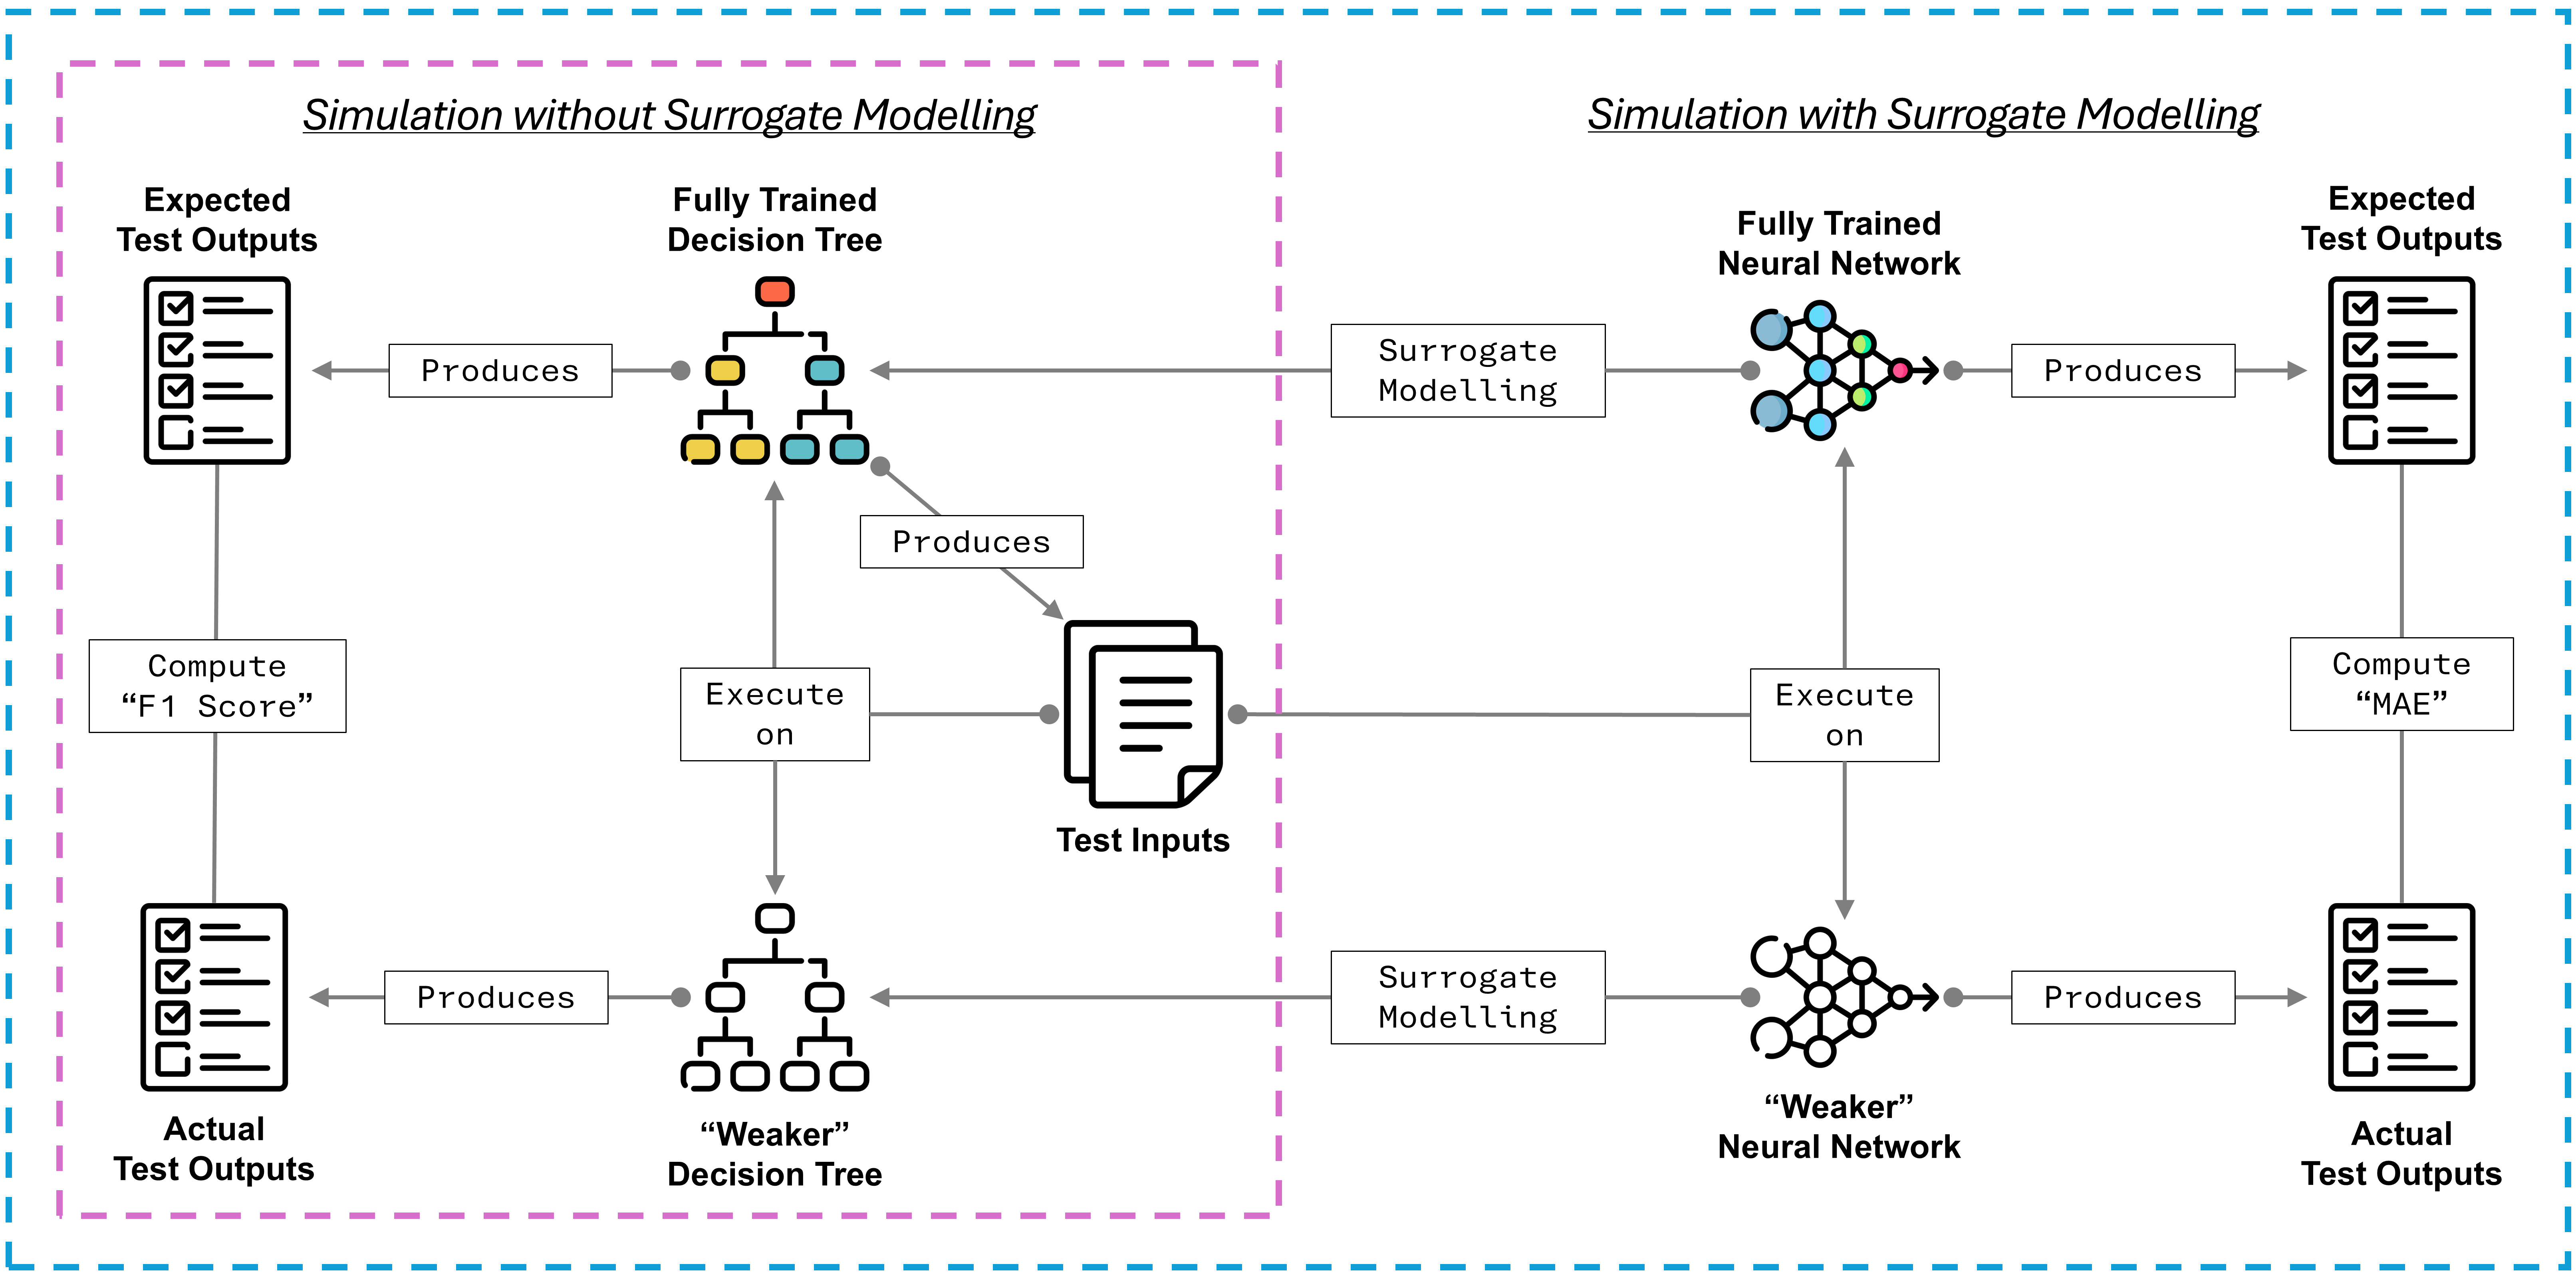
\includegraphics[width=\linewidth]{img/simulationsetup}
\caption{Simulation workflow for evaluating the effectiveness of test inputs generated by our framework on a single dataset.}
\label{fig:simflow}
\end{figure}

%TODO # test inputs
\paragraph{Workflow.} To evaluate the effectiveness of the test inputs generated by our framework, we conduct two distinct simulation procedures. Figure~\ref{fig:simflow} illustrates the workflow for both simulations.

In the first simulation, we train two decision tree classifiers: one using the full dataset, and a second, referred to as the “weaker” model, using only 50\% of the same dataset. The decision tree trained on the full dataset is assumed to produce the “expected” test outcomes for any given input. The aim of this simulation is to assess how effectively the generated test inputs challenge the weaker model, thereby revealing its reduced accuracy due to limited training data. The fully trained decision tree is provided to our framework as the input data-driven model, from which test inputs are subsequently generated. These inputs are executed on both the full and weaker decision trees, producing two sets of test outputs. We compare the expected outputs from the full model with the actual outputs from the weaker model using the F\textsubscript{1} score. The F\textsubscript{1} score is a widely adopted metric for evaluating the performance of classification models, particularly in scenarios involving imbalanced class distributions~\cite{mlbook}. While alternative metrics exist, we consider the F\textsubscript{1} score the most suitable for evaluating the effectiveness of test inputs, as it captures the ability of a model to correctly identify true positives while minimising false positives and false negatives. By comparing F\textsubscript{1} scores across different test input generation strategies, we assess how effectively each strategy exposes both correct and incorrect classifications made by the weaker model.

In the second simulation, we follow a similar procedure using neural networks. One network is trained on the full dataset, while the weaker network is trained on 50\% of the same data. As before, the full model is assumed to produce the expected test outcomes. The goal is to evaluate how well the generated test inputs expose the limitations of the weaker neural network. The fully trained neural network is provided to our framework as the input data-driven model. The framework applies surrogate modelling, as described in Section~\ref{sec:surrogate}, to learn a decision tree that approximates the behaviour of the neural network. Test inputs are generated from this surrogate model and executed on both the full and weaker neural networks, yielding two sets of test outputs. We compare these outputs using the MAE, a standard metric for evaluating the performance of regression models. Although other metrics are available, MAE is particularly suitable here as it quantifies the average magnitude of error between expected and actual outputs. By comparing MAE values across different test input generation strategies, we determine how effectively each strategy reveals prediction errors in the weaker model.

We apply the first simulation to all datasets used for classification tasks, as listed in Table~\ref{tab:cladata}, and the second simulation to those used for regression tasks, shown in Table~\ref{tab:regdata}. For each simulation run, the framework is executed four times, each with a distinct test requirement (TR):
\begin{enumerate}[align=left]
\item[\textbf{TR1:}] DTC (Definition~\ref{def:dtc}) with the proportional test allocation strategy (Definition~\ref{def:prop}), referred to as DTC Proportional.
\item[\textbf{TR2:}] DTC with the inverse test allocation strategy (Definition~\ref{def:inverse}), referred to as DTC Inverse.
\item[\textbf{TR3:}] BVA (Definition~\ref{def:bva}) with the proportional test allocation strategy, referred to as BVA Proportional.
\item[\textbf{TR4:}] BVA with the inverse test allocation strategy, referred to as BVA Inverse.
\end{enumerate}

In all cases, the framework is configured to generate a total of 5000 test inputs. The global range for each feature is determined using the observed minimum and maximum values within the respective dataset, rather than relying on manually specified feature ranges. For BVA-based executions, the neighbourhood size around boundary values is set to $\epsilon = 1.0$.

In addition to our framework, we generate test inputs for each dataset using four baseline methods. This results in four distinct sets of test inputs per dataset. For classification datasets, these inputs are executed on both the fully trained and weaker decision trees. For regression datasets, they are executed on the corresponding full and weaker neural networks. Each execution yields a set of expected and actual test outputs. Depending on the task type, we compute either the F\textsubscript{1} score or MAE for each pair of outputs. We compare these metrics across all test input generation strategies to assess the relative effectiveness of the generated test inputs.

%TODO # test inputs
\paragraph{Baselines.} We present four baseline methods for generating test inputs, which serve as reference points for evaluating those produced by our framework.
\begin{enumerate}
\item \textit{Random Sampling} (RS): Samples 5000 random values from the global range of each input feature, defined by the minimum and maximum values observed in the corresponding dataset. These values are then combined across features to form 5000 test inputs.
\item \textit{Boundary Sampling} (BS): Samples 5000 values from the neighbourhood around the upper and lower bounds of each global feature range, using a neighbourhood size of $\epsilon = 1.0$. These values are then combined across features to form 5000 test inputs. 
\item \textit{Quantile-Based Sampling} (QBS): Each feature range is divided into four intervals, also known as quantiles, each containing an equal portion of values from the dataset. From each quantile, 1250 synthetic values are generated and combined across features to form 5000 test inputs.
\item \textit{Example-Based Sampling} (EBS): Samples 5000 examples directly from the dataset to use as test inputs. Sampling is performed with replacement if the dataset contains fewer than 5000 instances, and without replacement otherwise.
\end{enumerate}

The first three baseline methods employ random sampling with varying levels of complexity, depending on how the sampling intervals are defined. RS is the simplest, relying on global feature ranges, whereas QBS is the most complex, using quantile-based partitions for each feature range. These methods are conceptually aligned with our framework, which also applies random sampling within equivalence class intervals and near their boundaries. The final baseline is a widely adopted strategy for generating test inputs to evaluate machine learning models, commonly used in techniques such as cross-validation and bootstrapping~\cite{durelli}.

\section{Evaluation}
\label{sec:res}

In this section, we analyse the simulation results comparing our framework against four baseline methods, with reference to the formulated hypotheses. We then evaluate the overall performance of our framework in generating effective test inputs and examine its limitations. Finally, we discuss potential threats to the validity of our research.
\subsection{Hypothesis Testing}

\subsubsection{Effectiveness of Test Inputs Without Surrogate Modeling}
\begin{figure}
\centering
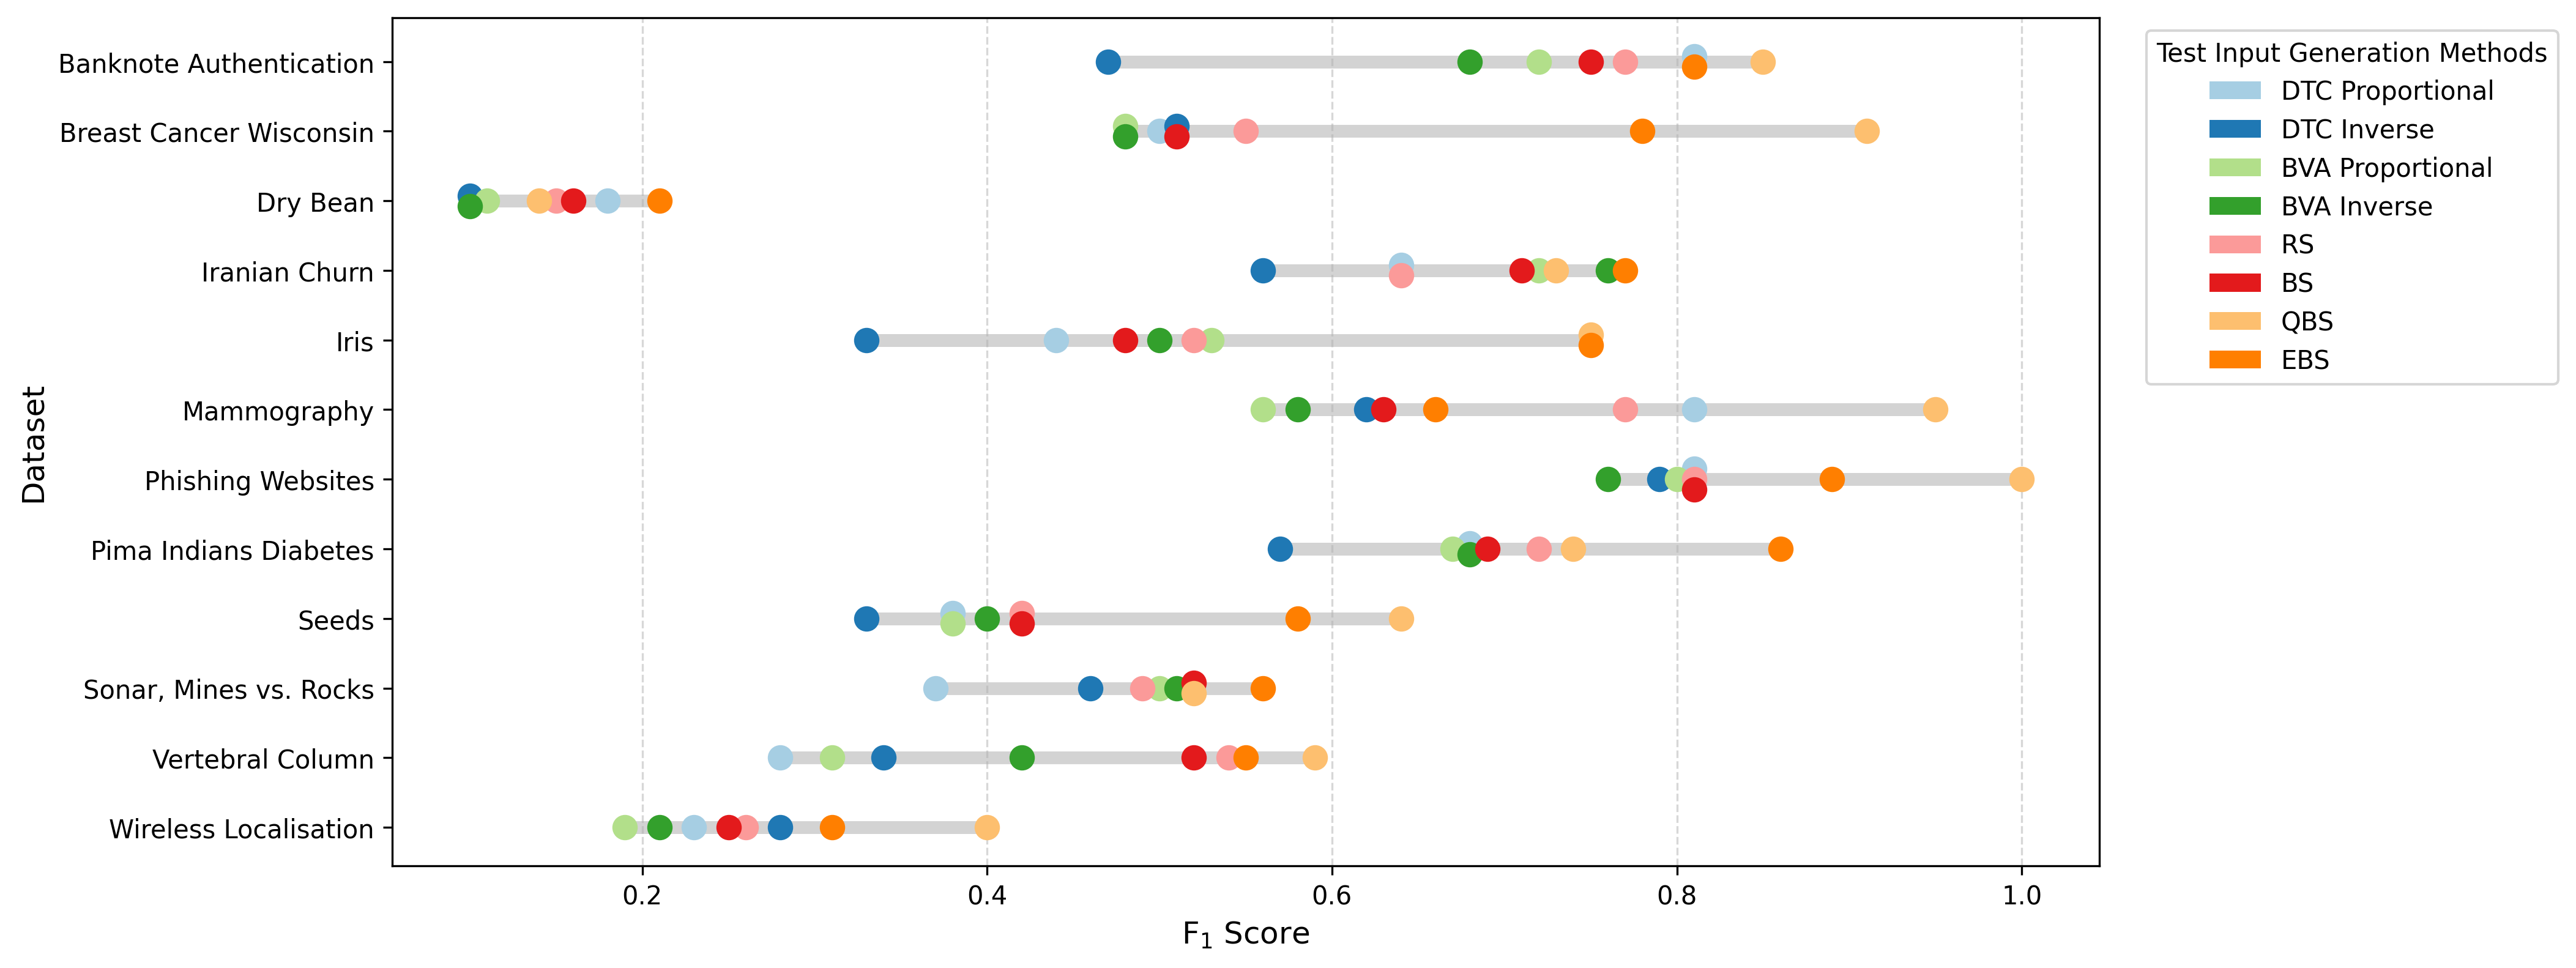
\includegraphics[width=\linewidth]{img/f1_score_plot}
\caption{Effectiveness comparison of test inputs generated by our framework and baseline methods in the first simulation. The x-axis shows the F\textsubscript{1} score, and the y-axis lists the datasets used for classification tasks (see Table~\ref{tab:cladata}). Each dot represents the F\textsubscript{1} score of test inputs generated either by our framework using one of four test requirements (DTC Proportional, DTC Inverse, BVA Proportional, BVA Inverse) or by one of four baseline methods (RS, BS, QBS, EBS).}
\label{fig:f1}
\end{figure}
Figure~\ref{fig:f1} presents the results of the first simulation using a connected dot plot. Each horizontal line corresponds to a classification dataset (see Table~\ref{tab:cladata}), and each dot represents the F\textsubscript{1} score obtained from a distinct set of test inputs executed on decision trees trained on that dataset. For each dataset, eight F\textsubscript{1} scores are shown. Four come from our framework under different test requirements, and four from the baseline methods (Section~\ref{sec:setup}). Identical scores within a dataset are stacked vertically with a slight offset.

Lower F\textsubscript{1} scores (dots positioned further left) indicate higher effectiveness in revealing model misclassifications, as defined in Definition~\ref{def:claeff}. Across all datasets, at least one configuration from our framework outperforms the baselines. Notably, no configuration performs worse than all baseline methods on any dataset.

However, performance varies across test requirements and datasets. This is due to how test inputs are allocated across different methods. Baseline methods sample uniformly across the global feature range or its partitions, giving equal chance to discover effective inputs. In contrast, our framework allocates test inputs based on the distribution of training examples across the leaves of decision trees. When effective test inputs lie in dominant classes, DTC Inverse may overlook them, whereas DTC Proportional is more likely to detect them. This pattern is evident in datasets such as "Wireless Localisation", where DTC Inverse configuration performs less effectively, but DTC Proportional consistently outperforms all baselines. Conversely, when effective inputs lie in less dominant classes, DTC Proportional may underperform, as seen in "Mammography", where DTC Inverse proves more effective.

A similar pattern is observed in BVA configurations. When effective inputs are near boundaries of dominant classes, BVA Inverse may miss them, while BVA Proportional is more likely to detect them. The reverse also occurs, where BVA Inverse outperforms BVA Proportional.

In "Solar, Mines vs Rocks", BVA configurations perform worse than RS, likely because effective test inputs lie within feature intervals rather than near boundaries. In such cases, DTC configurations yield better results. The opposite is also observed, where BVA configurations outperform other methods. This suggests that effective inputs lie near equivalence class boundaries rather than within intervals.

Overall, the simulation results partially support Hypothesis 1. Without surrogate modelling, our framework can generate more effective test inputs than baseline methods, but only when configured to target fault-prone regions of the input space. Under suitable test requirements, our approach can produce challenging inputs that expose system weaknesses beyond what simple random sampling achieves.

\subsubsection{Effectiveness of Test Inputs With Surrogate Modeling}
\begin{figure}
\centering
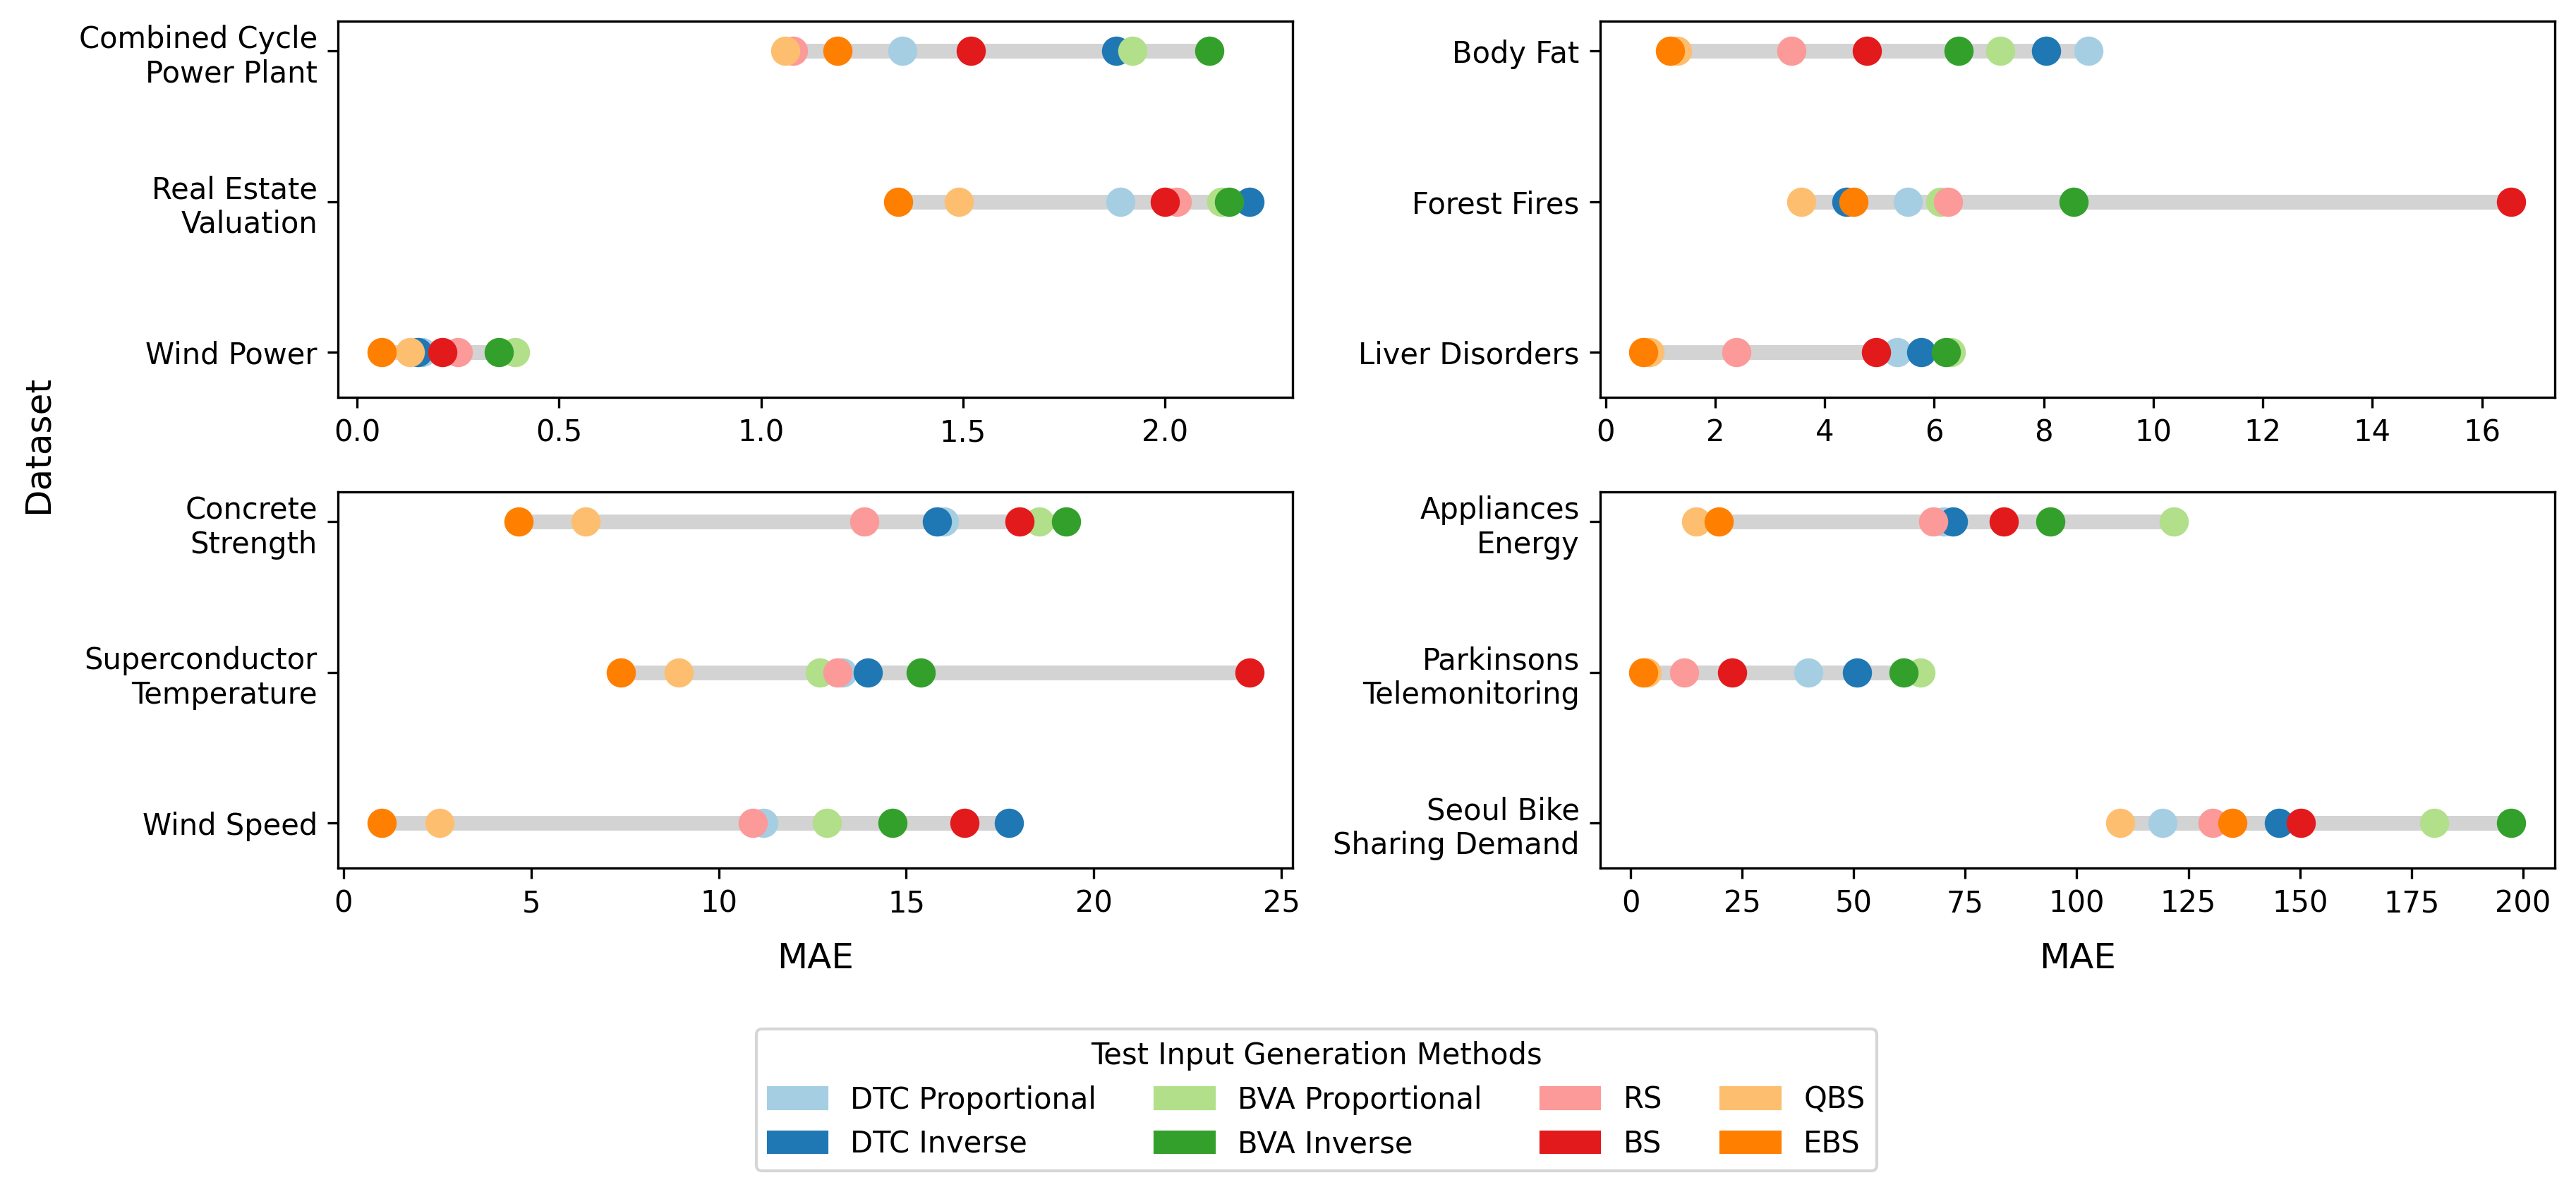
\includegraphics[width=\linewidth]{img/mae_plot}
\caption{Effectiveness comparison of test inputs generated by our framework and baseline methods in the second simulation. The figure consists of four plots, each displaying results for datasets with similar MAE scales. In all plots, the x-axis shows the MAE, and the y-axis lists the datasets used for regression tasks (see Table~\ref{tab:regdata}). Each dot represents the MAE obtained from test inputs generated either by our framework using one of four test requirements (DTC Proportional, DTC Inverse, BVA Proportional, BVA Inverse) or by one of four baseline methods (RS, BS, QBS, EBS).}
\label{fig:mae}
\end{figure}

Figure~\ref{fig:mae} presents the results of the second simulation using four connected dot plots. Each plot groups datasets with similar MAE scales. As in the first simulation, each horizontal line represents a regression dataset (see Table~\ref{tab:regdata}), and each dot shows the MAE score from test inputs generated either by our framework or by the baseline methods.

Unlike the F\textsubscript{1} score, lower MAE values (dots positioned further to the left) indicate lower effectiveness in revealing prediction errors, as defined in Definition~\ref{def:regeff}. In ten out of twelve datasets, at least one configuration from our framework outperforms the baselines. However, the most effective configuration varies across datasets due to differences in test input allocation strategy employed by each method, as discussed earlier. As also seen in the first simulation, the relative performance of DTC and BVA configurations depends on whether effective test inputs lie near equivalence class boundaries or within feature intervals.

A pattern not observed in the first simulation is that, for "Superconductor Temperature" and "Forest Fires", none of the configurations from our framework outperform BS. In both datasets, BS achieves significantly better results. This is likely because the most effective inputs are located at the boundaries of the global feature range. Our framework, particularly under BVA configurations, does not typically generate inputs from these regions, as such boundaries are rarely used in the split conditions of decision trees. Instead, it targets equivalence class boundaries, which usually lie within the feature range.

The second simulation results are partially consistent with Hypothesis 2. Our framework can outperform the baseline methods even when surrogate modelling is applied, given that the test requirements are appropriately configured. However, its performance declines when the most effective inputs are concentrated solely at the global boundaries.

\subsubsection{Input Space Coverage}
\begin{table}
\caption{Volumes of the MBB computed from all sets of test inputs across both simulations. Test inputs are generated either by our framework using one of four test requirements (DTC Proportional, DTC Inverse, BVA Proportional, BVA Inverse) or by one of four baseline methods (RS, BS, QBS, EBS).}
\label{tab:volume}
\resizebox{\textwidth}{!}{%
\begin{tabular}{lllllllll}\toprule
Dataset & DTC Proportional & DTC Inverse  & BVA Proportional & BVA Inverse & RS & BS & QBS & EBS \\\midrule
Banknote Authentication      &  \num{94409} & \num{94382} & \num{59908} & \num{58386} & \num{94380} & \num{149313} & \num{81539} & \num{94609} \\
Breast Cancer Wisconsin      &  \num{5.60e8} & \num{5.61e8} & \num{2.42e14} & \num{1.40e14} & \num{5.56e8} & \num{2.63e29} & \num{2.56e8} & \num{5.63e8} \\
Dry Bean                               &  \num{1.76e13} & \num{1.69e13} & \num{2.90e24} & \num{2.18e24} & \num{1.75e13} & \num{3.50e25} & \num{7.86e12} & \num{1.11e13} \\
Iranian Churn                        &  \num{1.21e21} & \num{1.20e21} & \num{1.21e21} & \num{9.60e20} & \num{1.21e21} & \num{7.05e22} & \num{0} & \num{1.20e21} \\
Iris                                         &  \num{132} & \num{131} & \num{150} & \num{148} & \num{122} & \num{855} & \num{114} & \num{122} \\
Mammography                     &  \num{3.91e6} & \num{3.81e6} & \num{8.05e5} & \num{8.14e5} & \num{3.90e6} & \num{1.32e7} & \num{3.08e6} & \num{1.99e6} \\
Phishing Websites                 &  \num{5.37e8} & \num{5.37e8} & \num{2.68e8} & \num{2.68e8} & \num{5.37e8} & \num{8.65e17} & \num{0} & \num{5.37e8} \\
Pima Indians Diabetes           &  \num{4.35e14} & \num{4.32e14} & \num{2.31e14} & \num{2.28e14} & \num{4.35e14} & \num{1.00e15} & \num{3.45e14} & \num{4.35e14} \\
Seeds                                     &  \num{220} & \num{220} & \num{10784} & \num{9832} & \num{219} & \num{90876} & \num{172} & \num{220} \\
Sonar, Mines vs. Rocks          &  \num{1.16e-22} & \num{1.16e-22} & \num{2.67e-11} & \num{2.84e-11} & \num{1.08e-22} & \num{9.73e24} & \num{1.44e-23} & \num{1.10e-22} \\
Vertebral Column                  &  \num{2.87e12} & \num{2.85e12} & \num{2.40e11} & \num{2.36e11} & \num{2.79e12} & \num{3.14e12} & \num{2.43e12} & \num{2.80e12} \\
Wireless Localisation             &  \num{2.70e11} & \num{2.70e11} & \num{4.57e10} & \num{4.38e10} & \num{2.70e11} & \num{3.77e11} & \num{2.11e11} & \num{2.62e11} \\
Appliances Energy                 &  \num{1.18e40} & \num{1.04e40} & \num{3.59e38} & \num{3.29e38} & \num{2.09e38} & \num{2.42e40} & \num{8.20e37} & \num{1.31e38} \\
Body Fat                                 &  \num{1.52e20} & \num{1.82e20} & \num{4.76e18} & \num{4.31e18} & \num{6.69e18} & \num{3.72e20} & \num{3.52e18} & \num{6.73e18} \\
Combined Cycle Power Plant &  \num{2.42e8} & \num{2.45e8} & \num{2.88e7} & \num{2.84e7} & \num{5.97e6} & \num{7.05e8} & \num{5.42e6} & \num{5.71e6} \\
Concrete Strength                  &  \num{8.30e19} & \num{8.86e19} & \num{2.75e15} & \num{2.67e15} & \num{6.32e18} & \num{1.39e20} & \num{4.18e18} & \num{6.34e18} \\
Forest Fires                            &  \num{1.75e16} & \num{1.72e16} & \num{2.66e14} & \num{2.61e14} & \num{9.15e15} & \num{3.21e25} & \num{0} & \num{9.17e15} \\
Liver Disorders                       &  \num{1.66e10} & \num{1.63e10} & \num{9.54e8} & \num{9.54e8} & \num{1.48e10} & \num{5.47e10} & \num{1.21e10} & \num{1.48e10} \\
Parkinsons Telemonitoring    &  \num{1.04e-2} & \num{1.02e-2} & \num{5.33e-5} & \num{5.26e-5} & \num{3.41e-6} & \num{6.00e11} & \num{2.11e-6} & \num{3.22e-6} \\
Real Estate Valuation             &  \num{19792} & \num{19945} & \num{14} & \num{14} & \num{19798} & \num{4.51e7} & \num{16465} & \num{19849} \\
Superconductor Temperature&  \num{3.01e160} & \num{2.90e160} & \num{8.98e158} & \num{8.31e158} & \num{1.00e160} & \num{3.37e166} & \num{6.36e158} & \num{4.66e158} \\
Seoul Bike Sharing Demand  & \num{3.57e14} & \num{3.50e14} & \num{4.27e10} & \num{4.19e10}  & \num{1.18e14} & \num{2.64e17} & \num{0} & \num{1.14e14} \\
Wind Power                           &  \num{1.18e15} & \num{1.18e15} & \num{3.82e14} & \num{3.83e14} & \num{8.50e14} & \num{2.24e15} & \num{7.23e14} & \num{3.67e14} \\
Wind Speed                          &  \num{4.15e7} & \num{4.11e7} & \num{1.76e6} & \num{1.00e6} & \num{3.73e7} & \num{2.36e8} & \num{2.55e7} & \num{2.48e7} \\\bottomrule
\end{tabular}}
\end{table}

\begin{figure}
\centering
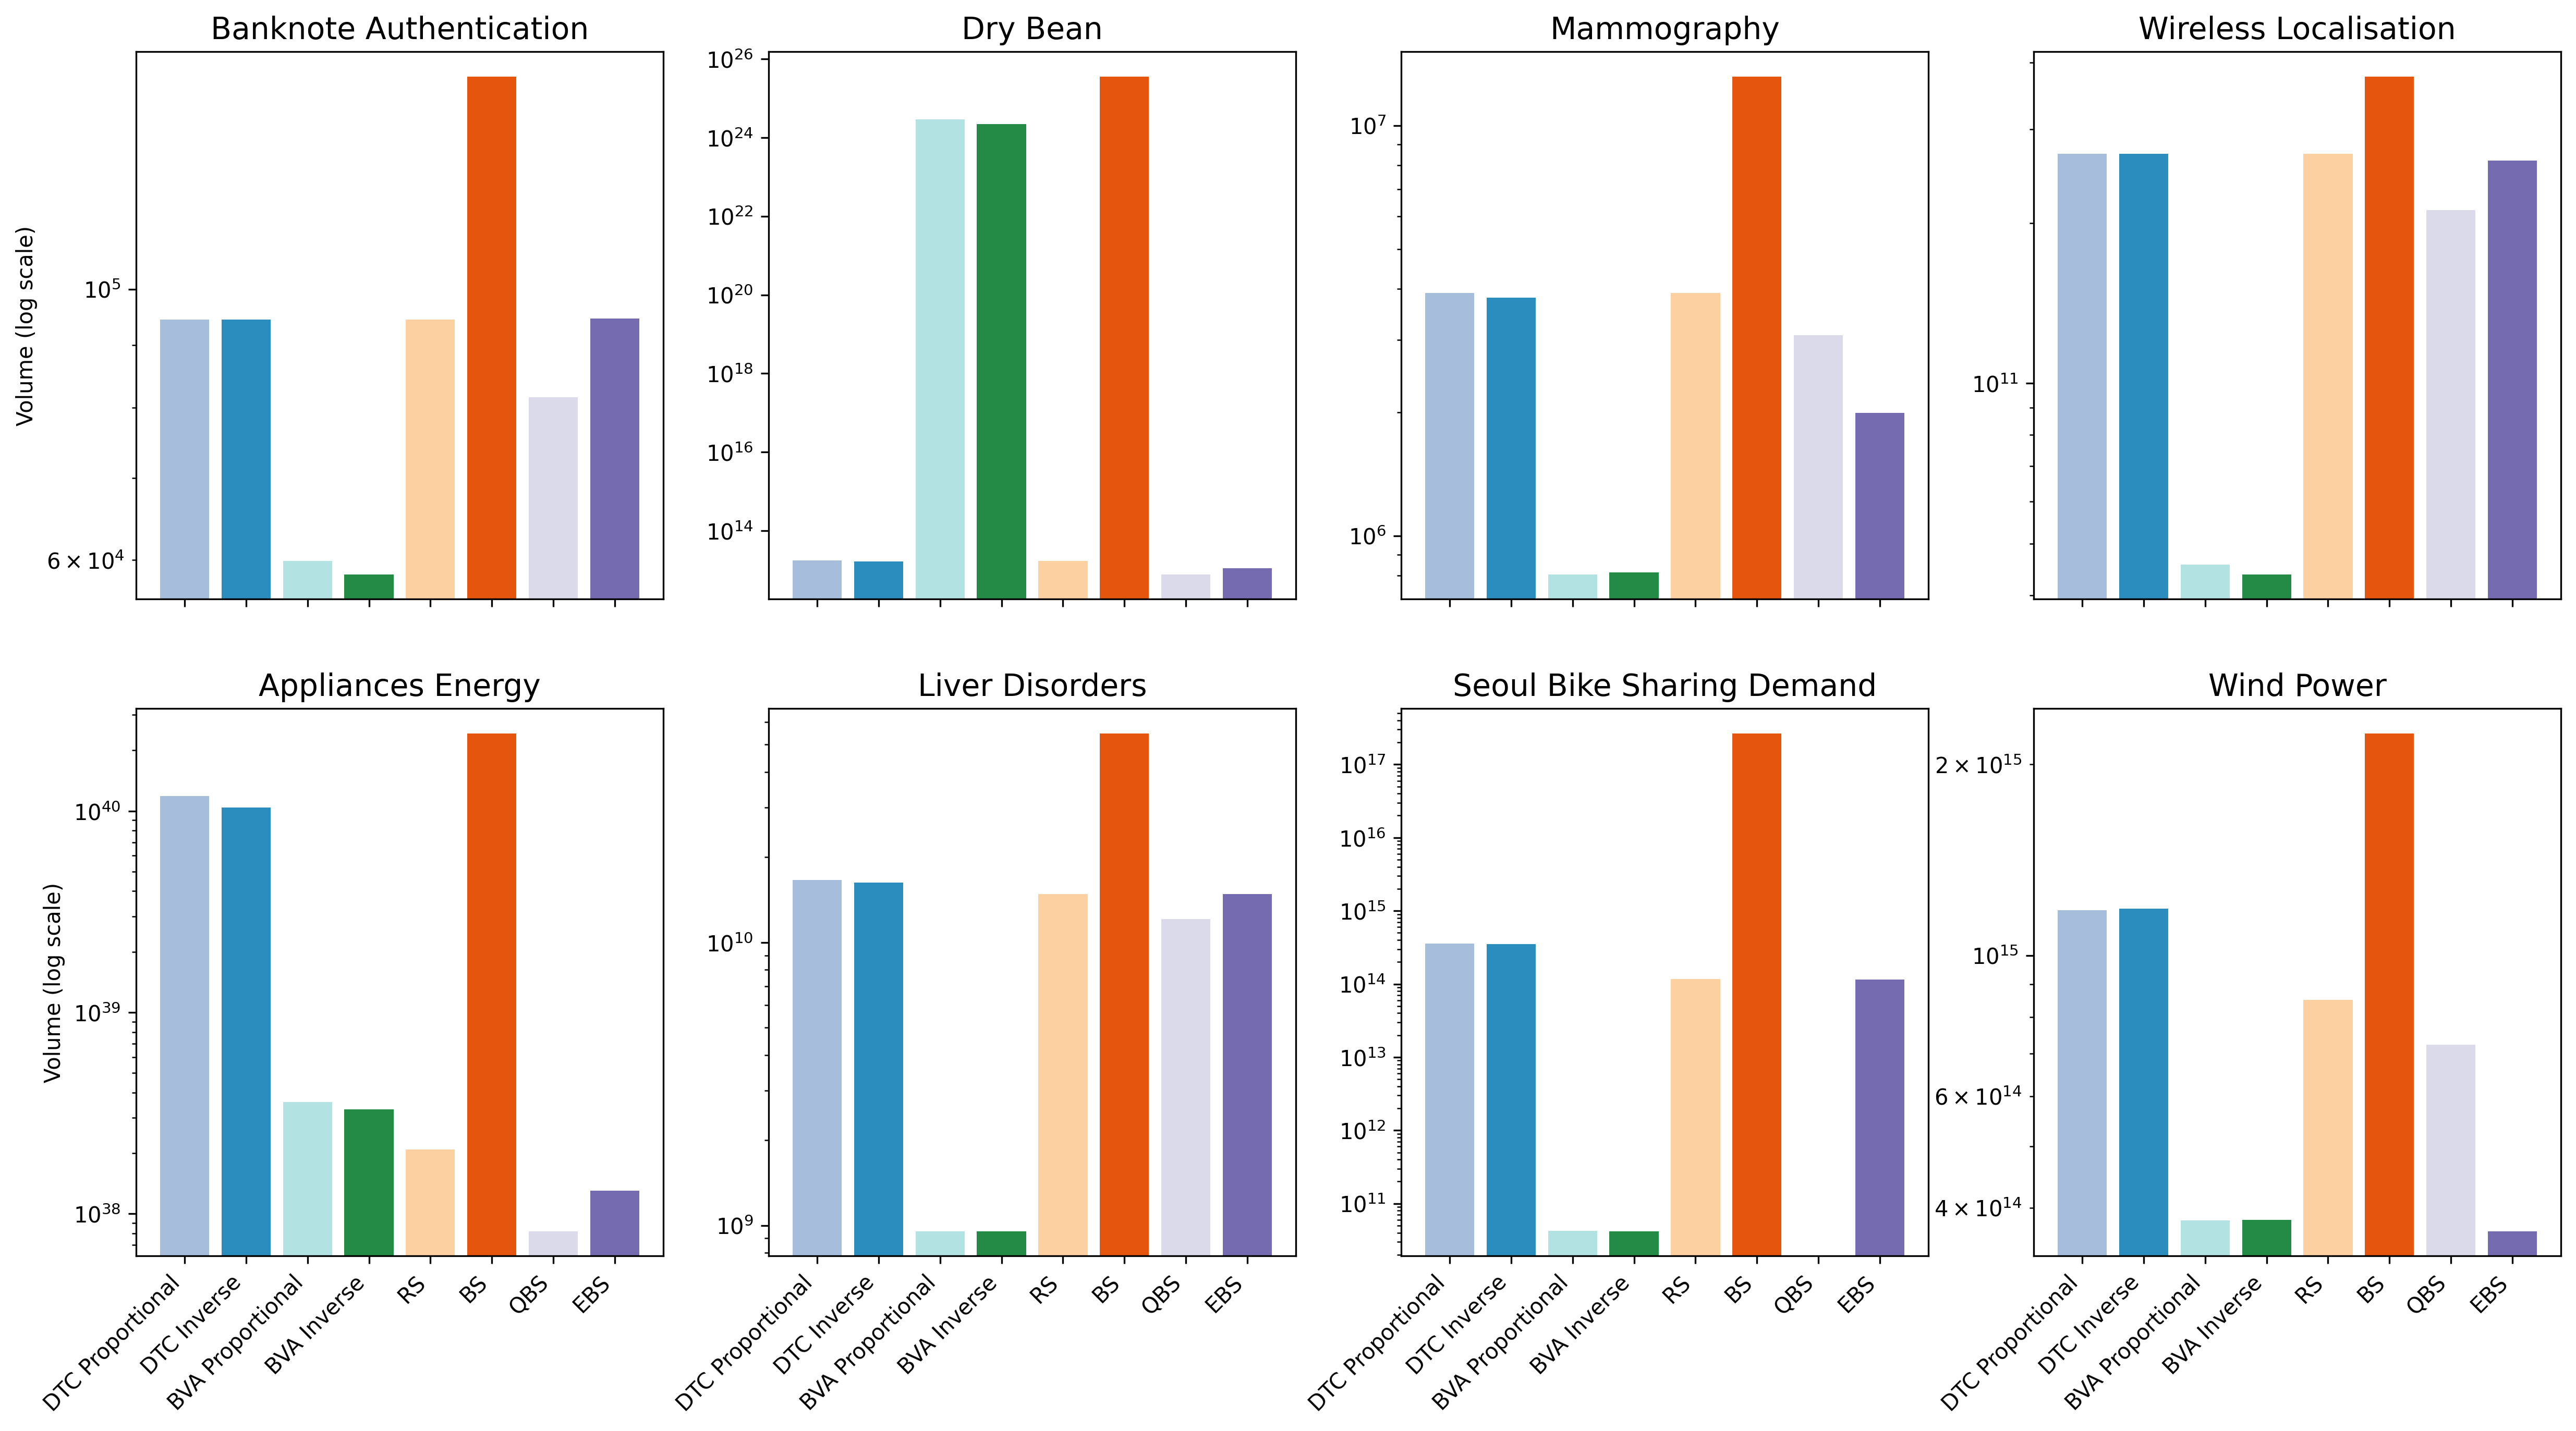
\includegraphics[width=\linewidth]{img/volume_plot}
\caption{Comparison of input space coverage by different sets of test inputs across both simulations. The figure comprises eight bar charts, showing results from representative datasets selected to highlight key patterns and differences. In every plot, bars indicate the volume of the MBB (as defined in Definition~\ref{def:mbb}), displayed on a logarithmic scale.}
\label{fig:volume}
\end{figure}

Table~\ref{tab:volume} presents the volumes of the MBB (see Definition~\ref{def:mbb}), calculated from all sets of test inputs across both simulations. These volumes indicate the extent of input space coverage achieved by each set. The test inputs are generated either by our framework or by one of four baseline methods. Based on these results, we select eight representative datasets and visualise their volumes in Figure~\ref{fig:volume}. Each chart in the figure displays the corresponding MBB volume on a logarithmic scale.

Across all datasets, BS consistently achieves the highest input space coverage. This is because BS samples test inputs around both the lower and upper bounds of each global feature range. Since all methods operate over a uniform global range, BS inherently covers the full input space by design.

The DTC and BVA configurations yield identical input space coverage within their respective pairs. This behaviour is consistent with the design, as each pair samples from the same equivalence class structure, either within the intervals or around the boundaries, but applies different allocation strategies to distribute test inputs.

DTC configurations generally achieve comparable or significantly greater coverage than RS, QBS, and EBS. RS and EBS rely on random sampling, which may fail to include test inputs spanning the entire space. While QBS divides the global feature range into quantiles and samples evenly across them, our framework leverages the internal structure of decision trees to define equivalence classes. This enables more granular and systematic coverage of the input space.

BVA configurations typically result in lower coverage than DTC. This is because BVA targets inputs only around equivalence class boundaries defined by the split conditions of the decision tree. As a result, test inputs may be generated around either the lower or upper bounds of intervals, but not both, leading to reduced overall coverage. An exception is observed in "Dry Bean", where BVA configurations outperform all methods except BS and achieve coverage comparable to BS. This is likely due to the decision tree defining boundaries near both ends of the global feature range, allowing BVA to sample more broadly.

These results partially support Hypothesis 3. In most cases, DTC configurations within our framework generate test inputs that cover a larger portion of the input space than RS, QBS, and EBS. BVA configurations can achieve high coverage only when decision tree splits are positioned near both ends of the global feature range.

\subsubsection{Dispersion of Test Inputs}
\begin{figure}
\centering
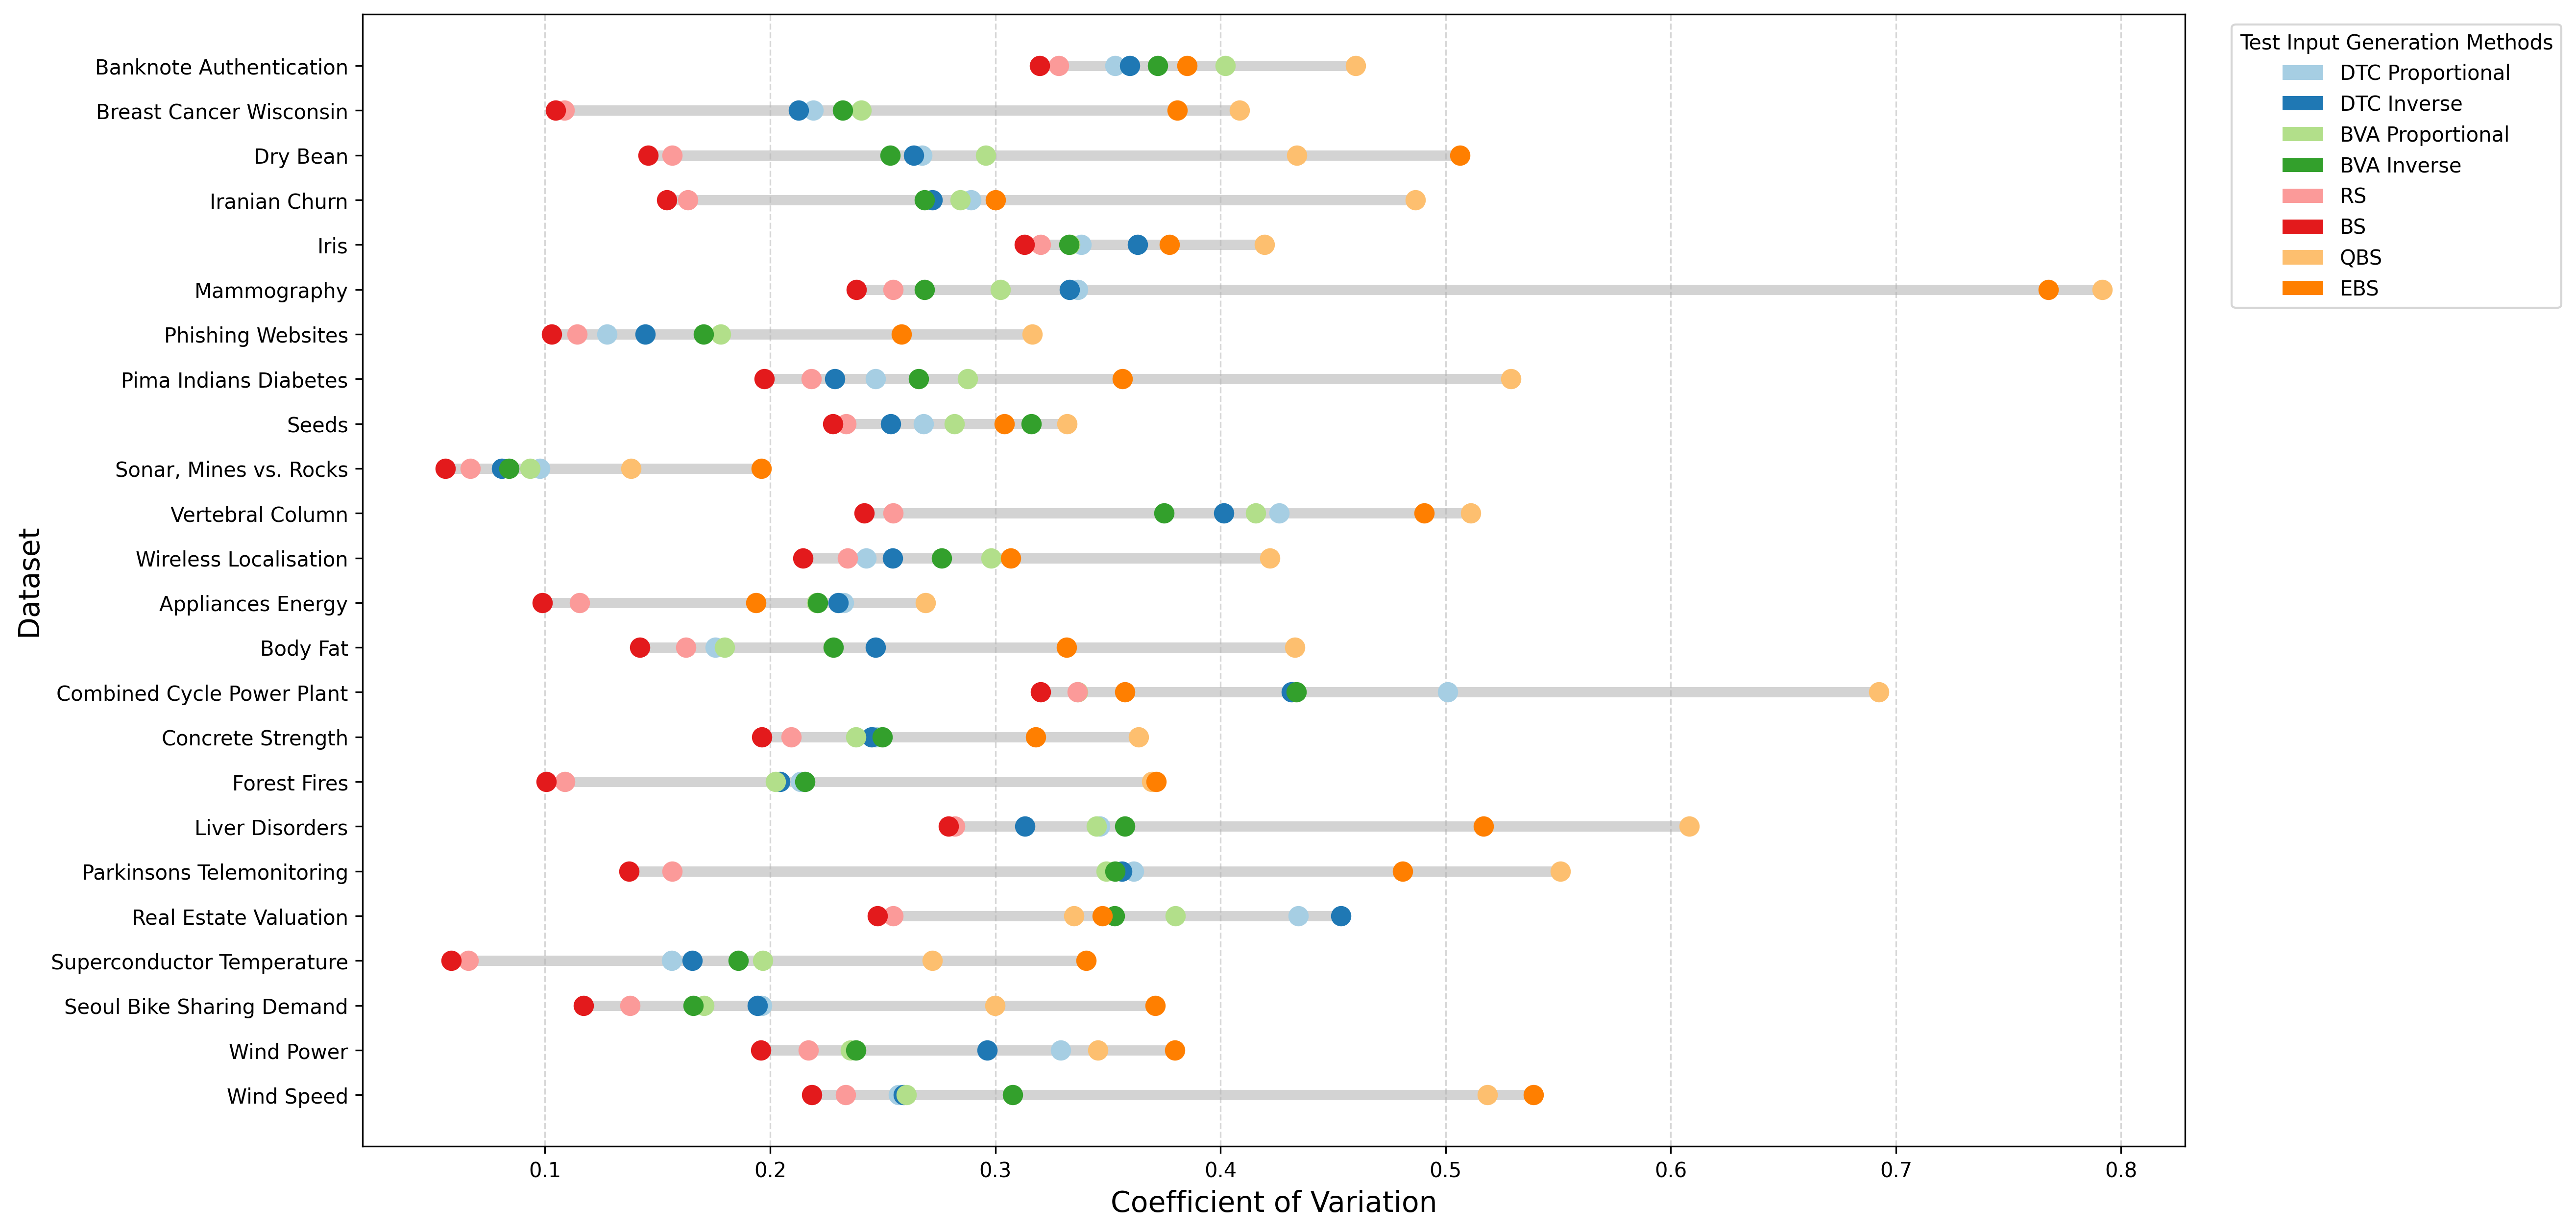
\includegraphics[width=\linewidth]{img/cv_plot}
\caption{Comparison of the dispersion of test inputs within the covered input space across both simulations. The x-axis shows the CV, and the y-axis lists the datasets. Each dot represents the CV for a given dataset, calculated from test inputs generated either by our framework, using one of four test requirements (DTC Proportional, DTC Inverse, BVA Proportional, BVA Inverse) or by one of four baseline methods (RS, BS, QBS, EBS).}
\label{fig:cv}
\end{figure}

Figure~\ref{fig:cv} presents a connected dot plot comparing the CV across test input sets from both simulations. Each horizontal line represents a distinct dataset, with dots indicating the CV calculated from inputs generated either by our framework or by one of the baseline methods.

The CV quantifies the relative variability of a distribution with respect to its mean, indicating how test inputs are spread within the covered input space. As defined in Definition~\ref{def:cv}, a higher CV (dots positioned further to the right) reflects greater variability, suggesting that test inputs are more widely scattered across different regions of the input space.

From the figure, we observe that BS consistently underperforms compared to other methods. BS generates inputs only near the boundaries of each global feature range. While this may produce a balanced distribution around the mean, it leaves large portions of the input space untested, resulting in low variability and a lower CV.

RS yields the second-lowest CV values among all methods. Although it samples uniformly across each global feature range, the resulting test inputs tend to cluster around the mean, leaving boundary regions sparsely populated~\cite{giraud}. This effect, explained by the law of large numbers, becomes more evident in high-dimensional spaces due to the curse of dimensionality. As a result, RS exhibits lower variability, indicating that its test inputs are less dispersed across the input space. The effect extends across datasets, as those with more features (i.e., higher-dimensional input spaces) tend to yield lower CV values under RS compared to datasets with fewer features.

Our framework consistently produces higher CVs than both RS and BS. This is because it partitions the input space into equivalence classes and samples test inputs from each class or around their boundaries. This strategy ensures broader coverage and greater dispersion, leading to more scattered inputs across the input space.

However, our framework does not outperform QBS in most datasets. This is due to differences in the test allocation strategy. Our framework allocates more inputs to either dominant or less dominant equivalence classes, depending on the chosen strategy. This causes clustering around specific regions, shifting the mean and reducing variability. Although inputs are still sampled from other classes, they are included less frequently. This contributes to increased variability, but not to the extent achieved by QBS. In contrast, QBS selects inputs from evenly spaced quantiles across the entire feature range, resulting in consistent dispersion and a higher CV. If training examples are distributed evenly across the leaf nodes, our framework generates a similar number of inputs per equivalence class. In such cases, it can yield a higher CV than QBS.

EBS generally yields high CV values, though its performance varies across datasets. For example, in "Combined Cycle Power Plant", EBS produces a lower CV than our framework. This variability stems from EBS sampling directly from the dataset, meaning the dispersion of test inputs reflects the underlying data distribution. If the dataset is widely scattered across the input space, the resulting CV will be high. If the data is concentrated in a specific region, the CV will be lower.

These findings support Hypothesis 4. Test inputs generated by our framework are scattered across the covered input space in a way that aligns with the proposed test allocation strategies. This is shown by their CV values, which are consistently higher than those of BS and RS, but lower than those achieved by QBS.

\subsection{Discussion}

The simulation results show that, across all evaluation criteria, the most effective test configuration within our framework varies depending on the dataset. This suggests that, while the framework is applicable to a range of data-driven models, it also exhibits flexibility. Specifically, by adjusting the test requirements, the framework can be tailored to generate test inputs that target fault-prone regions within the input domain of each SUT. These targeted inputs help uncover potential weaknesses in the system. However, if such regions lie near the boundaries of the global feature range, the framework may fail to produce inputs that effectively expose them, allowing certain faults to go undetected.

An aspect not reflected in the simulation results is the framework’s dependence on the quality of the data-driven models used to generate test inputs. For the framework to perform effectively, the data-driven models must either be decision trees with split conditions that accurately predict output labels at the leaves, or models that can be reliably approximated by tree surrogates with equally precise split conditions. These split conditions are essential for defining equivalence classes used in sampling test inputs. If the splits are poorly defined, the resulting classes may fail to represent meaningful regions of the input space that are processed similarly by the SUT. In such cases, fault-prone areas may not be properly isolated, and test inputs drawn from these classes may fail to reveal system weaknesses.

Another limitation is the framework’s inability to distinguish between time-series and non-time series data. Although time-series patterns are common in CPSs, the framework does not account for explicit model specifications related to temporal behaviour. It treats all input data as independent, ignoring any time-dependent structure. To ensure reliable test input generation, the underlying data-driven model must first transform any existing time-series dynamics into independent, non-sequential data before being passed to the framework.

Despite these considerations, the framework offers a reliable and structured approach to system evaluation, allowing thorough exploration of system boundaries and limitations. This is particularly useful in CPSs, where edge cases and uncommon scenarios can have a significant impact on their performance~\cite{survey}.

One practical use of the framework is in regression testing. As the system evolves through software updates, hardware modifications, or environmental shifts, it is crucial to ensure that existing functionality is preserved. The framework allows testers to generate inputs from a nominal system and execute them on both the original and updated systems. By comparing the test outputs using a common metric, testers can determine whether stability or performance of the SUT has been affected by the changes.

\subsection{Threats to Validity}

One potential threat to external validity is that the datasets used in our simulations may not reflect the input-output behaviour of real-world CPSs. These datasets are typically cleaner and less complex than those encountered in practice. As a result, it is possible that different outcomes might have observed had we used larger, more complex datasets collected from actual physical systems.

A threat to construct validity arises from the possibility that the evaluation metrics employed may not fully capture the effects we intended to investigate~\cite{durelli}. Although F1 score and MAE are standard measures for assessing machine learning models, they may not adequately reflect the quality of test inputs in the context of CPSs. Nonetheless, these metrics provide a clear and interpretable means of evaluating how effectively the inputs challenge the SUT, particularly in exploring edge cases and uncommon scenarios.

Other metrics could potentially be used to evaluate input space coverage and the dispersion of test inputs, besides bounding box volume and the CV. However, these two align well with the purpose of our analysis. Bounding box volume indicates how much of the input space is covered, while CV shows how spread out the inputs are within that space. Their definitions and calculation methods make them suitable choices for assessing these aspects.

Finally, another threat to construct validity may stem from potential faults in the implementation of our framework. Any such issues could affect the accuracy of the results and the reliability of the conclusions drawn.

\section{Concluding Remarks}
\label{sec:end}

Cyber-Physical Systems~(CPSs) are inherently large-scale and complex due to their integration of computing, communication, and control technologies. Rigorous testing is essential prior to deployment to ensure system reliability and safety. However, testing CPSs is challenging due to the difficulty of translating abstract requirements into concrete test inputs and accurately representing complex system behaviour.

To address these challenges, we introduce a test input generation framework based on data-driven models of CPSs. These models, constructed from system-generated data, reflect the behaviour of the physical system. By utilising data-driven models, the framework removes the burden of manually analysing or interpreting abstract requirements, as such requirements are implicitly encoded within the data. Furthermore, data-driven modelling eliminates the need for specific domain expertise, making the testing process more accessible. Our framework employs decision trees as white-box models to guide test input generation. Specifically, it partitions the input domain of the SUT into equivalence classes, derived from the tree’s internal structure. Test inputs are then statistically sampled from each class based on test requirements specified by the users. Additionally, we propose a method for training a decision tree surrogate from a data-driven model, allowing the same testing strategy to be applied across different model types. 

Simulation results show that, by adjusting the test requirements, our framework can be flexibly adapted to each SUT, allowing the generation of challenging inputs that effectively stress the system. These inputs span a broad range of values and are strategically dispersed throughout the input space, ensuring targeted and comprehensive exploration.

The framework generates test inputs offline, meaning all inputs are created in advance based on the test requirements before execution on the SUT. Offline generation offers several advantages: it allows for faster execution and enables pre-analysis of test coverage~\cite{hessel}. As part of future work, we explore model-based online testing, which combines input generation and execution in real time. In this approach, the test generator interactively stimulates and observes the SUT. Only a single input is generated from the model at a time, which is immediately executed on the SUT, and the resulting output is checked against the system specification. This process repeats until the test concludes or an error is detected. The method supports dynamic adaptation of test requirements and facilitates the automatic identification of fault-prone regions within the input space that require further exploration. However, online testing is more complex, particularly for CPSs, as it demands interpretation of system specifications and precise output evaluation. This requires embedded domain knowledge, which is difficult to integrate due to the complex and technically diverse nature of CPSs, involving real-time constraints and tightly coupled physical and digital components.

In addition to online testing, we plan to investigate alternative white-box surrogate models for test input generation. One promising candidate is the random forest, a machine learning model that aggregates the outputs of multiple decision trees to produce a single prediction~\cite{randomforest}. Random forests offer multiple options for partitioning the input space into equivalence classes. This flexibility allows us to select the most meaningful partitioning, where each class accurately represents a region of the input space processed similarly by the SUT. Moreover, by combining equivalence class partitions across different trees within the forest, the framework can construct an optimal structure for generating highly effective test inputs. This direction opens new possibilities for enhancing the precision and adaptability of our framework.


%% Formulation
% MUT, SUT?
% Abalone, Decision Tree?


%%
%% The acknowledgments section is defined using the "acknowledgments" environment
%% (and NOT an unnumbered section). This ensures the proper
%% identification of the section in the article metadata, and the
%% consistent spelling of the heading.
%\begin{acknowledgments}
%\end{acknowledgments}


%% The declaration on generative AI comes in effect
%% in Janary 2025. See also
%% https://ceur-ws.org/GenAI/Policy.html
\section*{Declaration on Generative AI}

  
\noindent During the preparation of this work, the authors used Microsoft Copilot in order to: Grammar and spelling check. After using the tool, the authors reviewed and edited the content as needed and takes full responsibility for the publication’s content. 


%%
%% Define the bibliography file to be used
\bibliography{paper-bib}


\end{document}

%%
%% End of file
